\documentclass[11pt,letterpaper,twoside]{book}

\usepackage[utf8]{inputenc}
\usepackage[spanish,es-tabla]{babel}
\decimalpoint
\let\cleardoublepage\clearpage
\usepackage[bitstream-charter]{mathdesign}
\usepackage[T1]{fontenc}
\newcommand{\selectSans}{\usefont{T1}{qhv}{m}{n}\selectfont} % sans-serif TeX Gyre Heros font
\usepackage{parskip}
\usepackage{amsmath}
\usepackage{amsfonts}
\usepackage{amssymb}
\usepackage{mathtools}
\usepackage{color}
\usepackage{graphicx}
\usepackage{makeidx}
\usepackage{pdflscape}
\makeindex
\usepackage{anysize}
\usepackage{anyfontsize}
\usepackage{pdfpages}
\usepackage[x11names,table]{xcolor}
\usepackage{tikz}
\usepackage{tcolorbox}
\tcbuselibrary{skins,breakable,listings,theorems}
\usepackage[hidelinks]{hyperref}
\usepackage[labelfont=bf]{caption}
\usepackage{subcaption}
\usepackage{float}
\captionsetup[table]{labelsep=space}
\captionsetup[figure]{labelsep=space}
\usepackage{setspace} % Para modificar espacios/interlineados
\usepackage{listings}
\usepackage{array,ragged2e}
\usepackage{multirow}
\usepackage{multicol}
\usepackage{enumitem}
% \usepackage{structuralanalysis}
\usepackage[titletoc]{appendix} % Para apéndices
\usepackage[left=2cm,top=2cm,right=2cm,bottom=2cm]{geometry}
\setlength{\parindent}{0cm}
\usepackage[printwatermark]{xwatermark}
\newwatermark[allpages,color=gray!10,angle=45,scale=3,xpos=0,ypos=0]{Borrador}
\tcbset{colback=green!5!white, colframe=gray!10!black, coltitle=green!20!black, 
fonttitle=\bfseries, colbacktitle=white, coltext=gray!30!black}
\addto\captionsspanish{
  \renewcommand{\figurename}{{\bf Figura}}% 
}
\addto\captionsspanish{
  \renewcommand{\chaptername}{{\bf}}% 
}
\usepackage{cancel}
\usepackage{textcomp}
\usepackage{gensymb}
\usepackage{newunicodechar}
\newunicodechar{°}{\degree}
\renewcommand{\vec}[1]{\boldsymbol{\mathbf{#1}}}
\renewcommand{\vecg}[1]{\boldsymbol{#1}}

\newcommand{\colvec}[3]{\begin{bmatrix}#1\\#2\\#3\end{bmatrix}}

\usepackage{epigraph}
\usepackage{fontawesome}
\usepackage[Bjornstrup]{fncychap}

\renewcommand{\baselinestretch}{1.00}
\newcommand{\hl}[1]{%
  \colorbox{red!50}{$\displaystyle#1$}} % Para cuadros colorizados

\newcommand{\answer}[1]{%
  \colorbox{green!50}{$\displaystyle#1$}} % Para cuadros colorizados
\newcommand{\sifu}[3]{\langle #1 - #2 \rangle^{#3}} % Funciones de singularidad

% \renewcommand{\familydefault}{\sfdefault}
\renewcommand{\vec}[1]{\mathbf{#1}}
\newcommand{\iszero}[1]{\cancelto{0}{#1}}




% Colores
\definecolor{verdep}{RGB}{166,206,58}
\definecolor{ccap}{RGB}{10,10,50}
\definecolor{csec}{RGB}{50,50,100}
\definecolor{csubsec}{RGB}{80,80,120}
\definecolor{header_table_color}{RGB}{200,255,180}
\definecolor{info_color}{RGB}{100,100,200}
\definecolor{csol}{rgb}{0.2,0.8,0.1}
\definecolor{backcode}{rgb}{0.98,0.98,0.99}
\definecolor{crule}{rgb}{0.9,0.9,0.9}
\definecolor{dkgreen}{rgb}{0,0.6,0}
\definecolor{gray}{rgb}{0.5,0.5,0.5}
\definecolor{mauve}{rgb}{0.58,0,0.82}
\definecolor{probsec}{RGB}{3,165,183}
\definecolor{codeinline}{RGB}{30,30,150}


% \newtcolorbox{ejemplo}[2][]
% {
%   breakable,
%   colframe = gray!100,
%   colback  = gray!0,
%   coltitle = gray!20!black,
%   title    =  \faEdit \hspace{5 mm} #2,
% }

\newcommand{\uno}{ ( \faStarO ) }
\newcommand{\dos}{ ( \faStarO\faStarO ) }
\newcommand{\tres}{ ( \faStarO\faStarO\faStarO ) }


\definecolor{extitle}{RGB}{0,50,0}
\definecolor{extitleback}{RGB}{225,225,225}
\definecolor{exback}{RGB}{255,255,255}
\definecolor{probtitleback}{RGB}{200,200,100}
\definecolor{probback}{RGB}{255,255,255}

\definecolor{solucolor}{RGB}{150,50,50}
\newcommand{\solu}{{\it\color{solucolor} Solución}}


\newtcolorbox[auto counter,number within=section]{ejemplo}[2][]{
  breakable,
  enhanced,
  colback=exback,
  boxrule=0.75pt,
  arc=6pt,
  % outer arc=0pt,
  title=\faEdit \hspace{5 mm}Ejemplo~\thetcbcounter \hspace{3mm} #2,
  fonttitle=\bfseries\sffamily\normalsize\strut,
  coltitle=extitle,
  colbacktitle=extitleback,
  % title style={exercisebgblue},
}

\newtcolorbox[auto counter,number within=section]{problema}[2][]{
  breakable,
  enhanced,
  colback=probback,
  boxrule=0.75pt,
  arc=6pt,
  % outer arc=0pt,
  title=\faEdit \hspace{5 mm}Problema~\thetcbcounter \hspace{3mm} #2,
  fonttitle=\bfseries\sffamily\normalsize\strut,
  coltitle=extitle,
  colbacktitle=extitleback,
  % title style={exercisebgblue},
}

\definecolor{infotitle}{RGB}{0,0,50}
\definecolor{infotitleback}{RGB}{195,240,255}
\definecolor{infoback}{RGB}{242,252,255}
\definecolor{infoframe}{RGB}{50,50,50}

\newtcolorbox{informacion}[2][]
{
  breakable,
  colframe = infoframe,
  colback  = infoback,
  coltitle = infotitle,
  colbacktitle = infotitleback,
  title    = \faInfo \hspace{5 mm} #2,
}

\newtcolorbox{recomendacion}[2][]
{
  breakable,
  colframe = green!25,
  colback  = green!10,
  coltitle = green!20!black,
  title    = #2,
}


% \newtcolorbox{outscript}[1][]
% {
%   breakable,
%   colframe = green!25,
%   colback  = green!10,
%   coltitle = green!20!black,
% }


\newcolumntype{P}[1]{>{\centering\arraybackslash}m{#1}}
\newcommand{\ccol}{>{\centering\tt\arraybackslash}}

% Nuevos comandos

\usepackage{titlesec}%--
% \newcommand{\hsp}{\hspace{5pt}}
% \titleformat{\chapter}[hang]{\huge\bfseries\color{ccap}}
% {\color{verdep}{\vrule height 2.5cm width 1mm}\hsp{\fontsize{100}{5}\selectfont\thechapter}\hsp%
% {\vrule height 2.5cm width 1mm}\hsp{\fontsize{30}{5}\selectfont}}{5pt}{\huge\bfseries}

\titleformat{\section}[hang]{\normalfont\color{csec}}%
{\filright\large\enspace\thesection\enspace}%
{8pt}{\Large\bfseries\filright}%

\titleformat{\subsection}[hang]{\normalfont\color{csec}}%
{\filright\large\enspace\thesubsection\enspace}%
{8pt}{\large\bfseries\filright}%


% For programming 
\newcommand{\code}[1]{{\tt\bfseries\color{codeinline} #1}}
\newcommand{\link}[1]{{\sffamily\color{codeinline}\url{#1}}}


% Code
\lstnewenvironment{python}{\lstset{frame=single,
  frameround=tttt,
  backgroundcolor=\color{backcode},
  rulecolor=\color{crule},
  language=python,
  aboveskip=4mm,
  belowskip=4mm,
  showstringspaces=false,
  columns=flexible,
  basicstyle={\small\ttfamily},
  numbers=none,
  numberstyle=\tiny\color{gray},
  keywordstyle=\color{blue},
  commentstyle=\color{dkgreen},
  stringstyle=\color{mauve},
  breaklines=true,
  breakatwhitespace=true,
  tabsize=4,
  extendedchars=true,
  inputencoding=utf8,
  literate=%
  {°}{{\,\,$^\circ$\,\,}}1
  {á}{{\'a}}1
  {é}{{\'e}}1
  {í}{{\'i}}1
  {ó}{{\'o}}1
  {ú}{{\'u}}1
  {Á}{{\'A}}1
  {É}{{\'E}}1
  {Í}{{\'I}}1
  {Ó}{{\'O}}1
  {Ú}{{\'U}}1
  {α}{{$alpha$}}1
  {₁}{{$ _1 $}}1
}}{}



\definecolor{backout}{RGB}{220,220,230}
\definecolor{textout}{RGB}{10,10,110}

% Code
\lstnewenvironment{outscript}{\lstset{frame=single,
  frameround=tttt,
  backgroundcolor=\color{backout},
  rulecolor=\color{crule},
  language=python,
  aboveskip=0mm,
  belowskip=4mm,
  showstringspaces=false,
  columns=flexible,
  basicstyle={\small\ttfamily\color{textout}},
  numbers=none,
  numberstyle=\tiny\color{gray},
  keywordstyle=\color{blue},
  commentstyle=\color{dkgreen},
  stringstyle=\color{mauve},
  breaklines=true,
  breakatwhitespace=true,
  tabsize=4,
  extendedchars=true,
  inputencoding=utf8,
  literate=%
  {°}{{\,\,$^\circ$\,\,}}1
  {á}{{\'a}}1
  {é}{{\'e}}1
  {í}{{\'i}}1
  {ó}{{\'o}}1
  {ú}{{\'u}}1
  {Á}{{\'A}}1
  {É}{{\'E}}1
  {Í}{{\'I}}1
  {Ó}{{\'O}}1
  {Ú}{{\'U}}1
  {α}{{$alpha$}}1
  {₁}{{$ _1 $}}1
}}{}



\author{
Pedro Jorge De Los Santos
}

\title{
% \vspace{-20mm}
{\normalsize Universidad Politécnica de Guanajuato} \\[-4mm]
{\normalsize Departamento de Ingeniería Robótica} \\
{\bfseries Una introducción a Python}
% 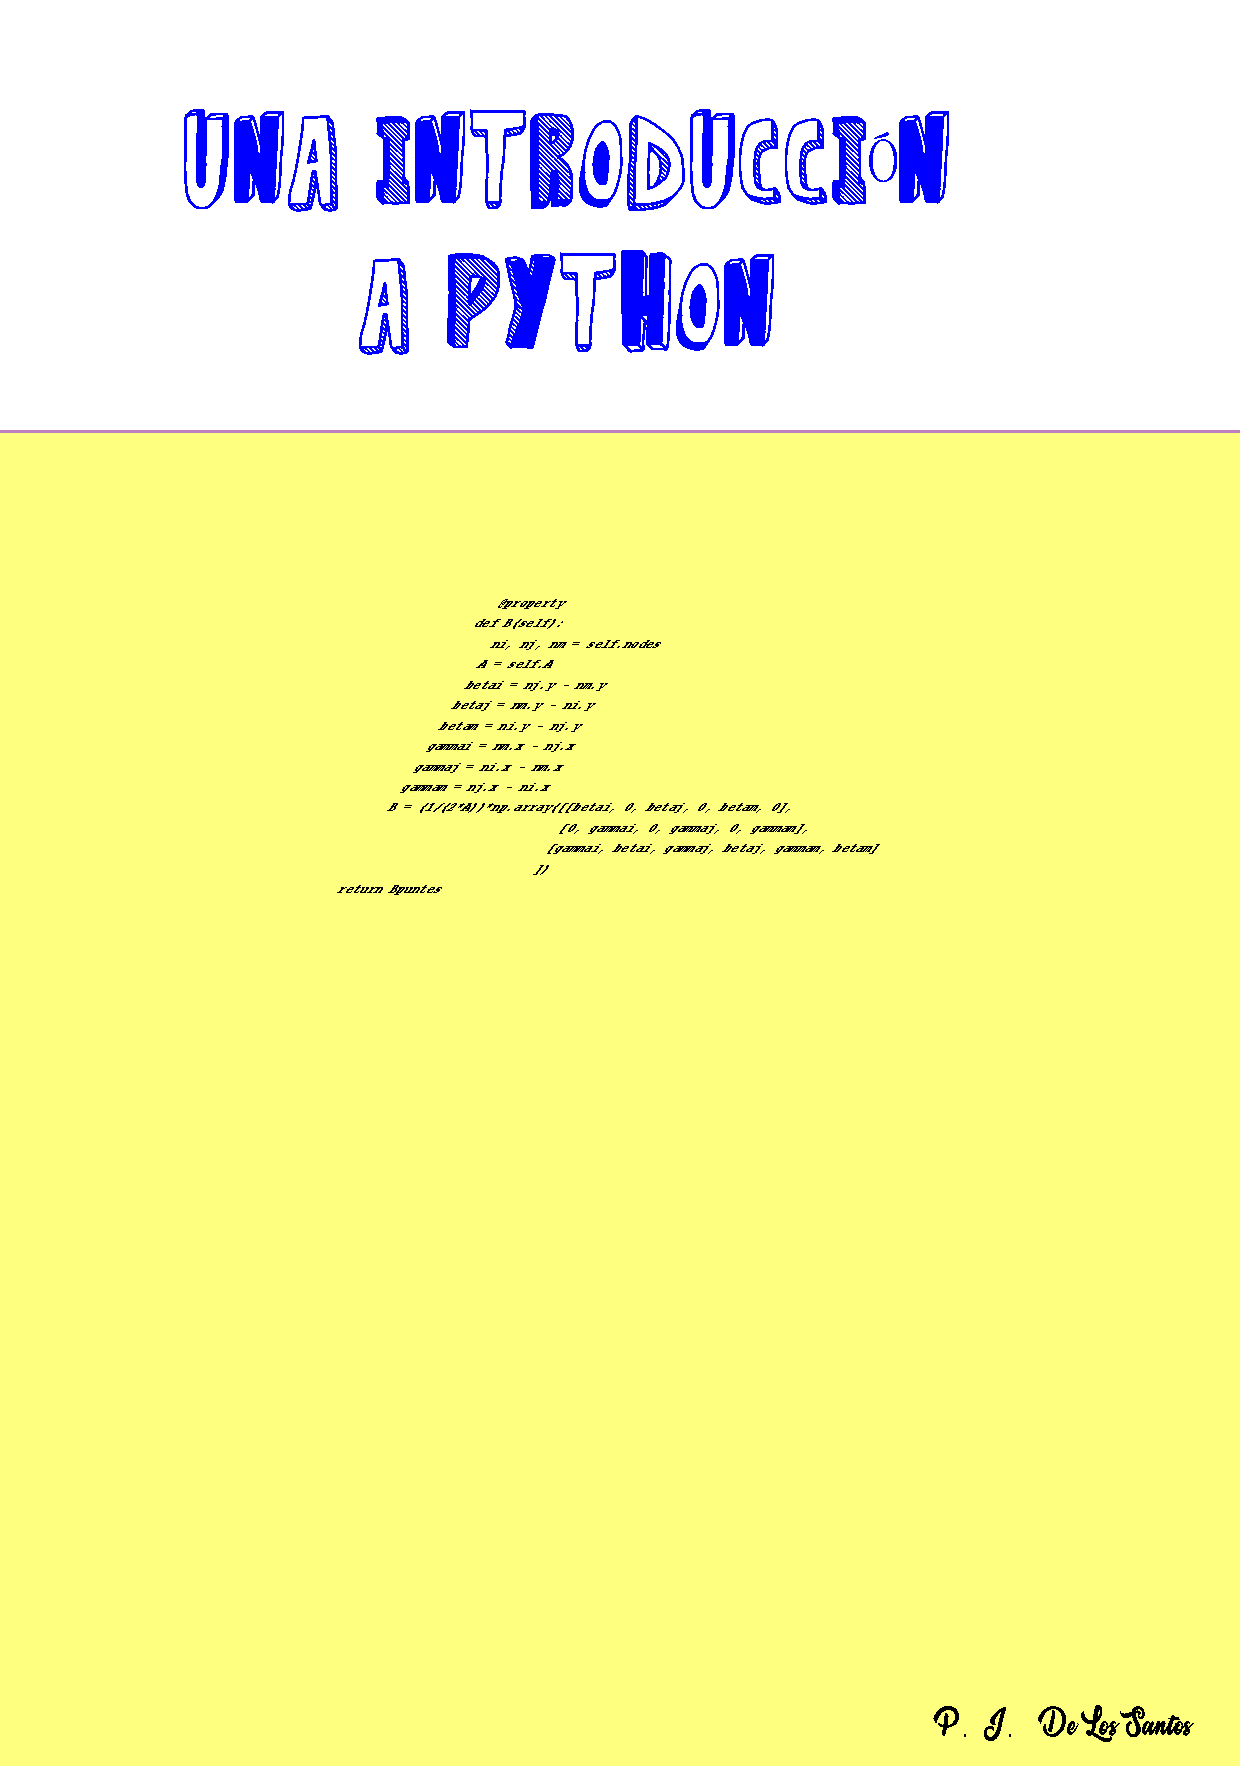
\includegraphics{img/cover.pdf}
}

% \date{}

% =================================================================
% =================================================================
%                              CONTENIDO
% =================================================================
% =================================================================

\begin{document}
% Config
% \setlength{\abovedisplayskip}{0pt}
% \setlength{\belowdisplayskip}{0pt}
% Contenido
% 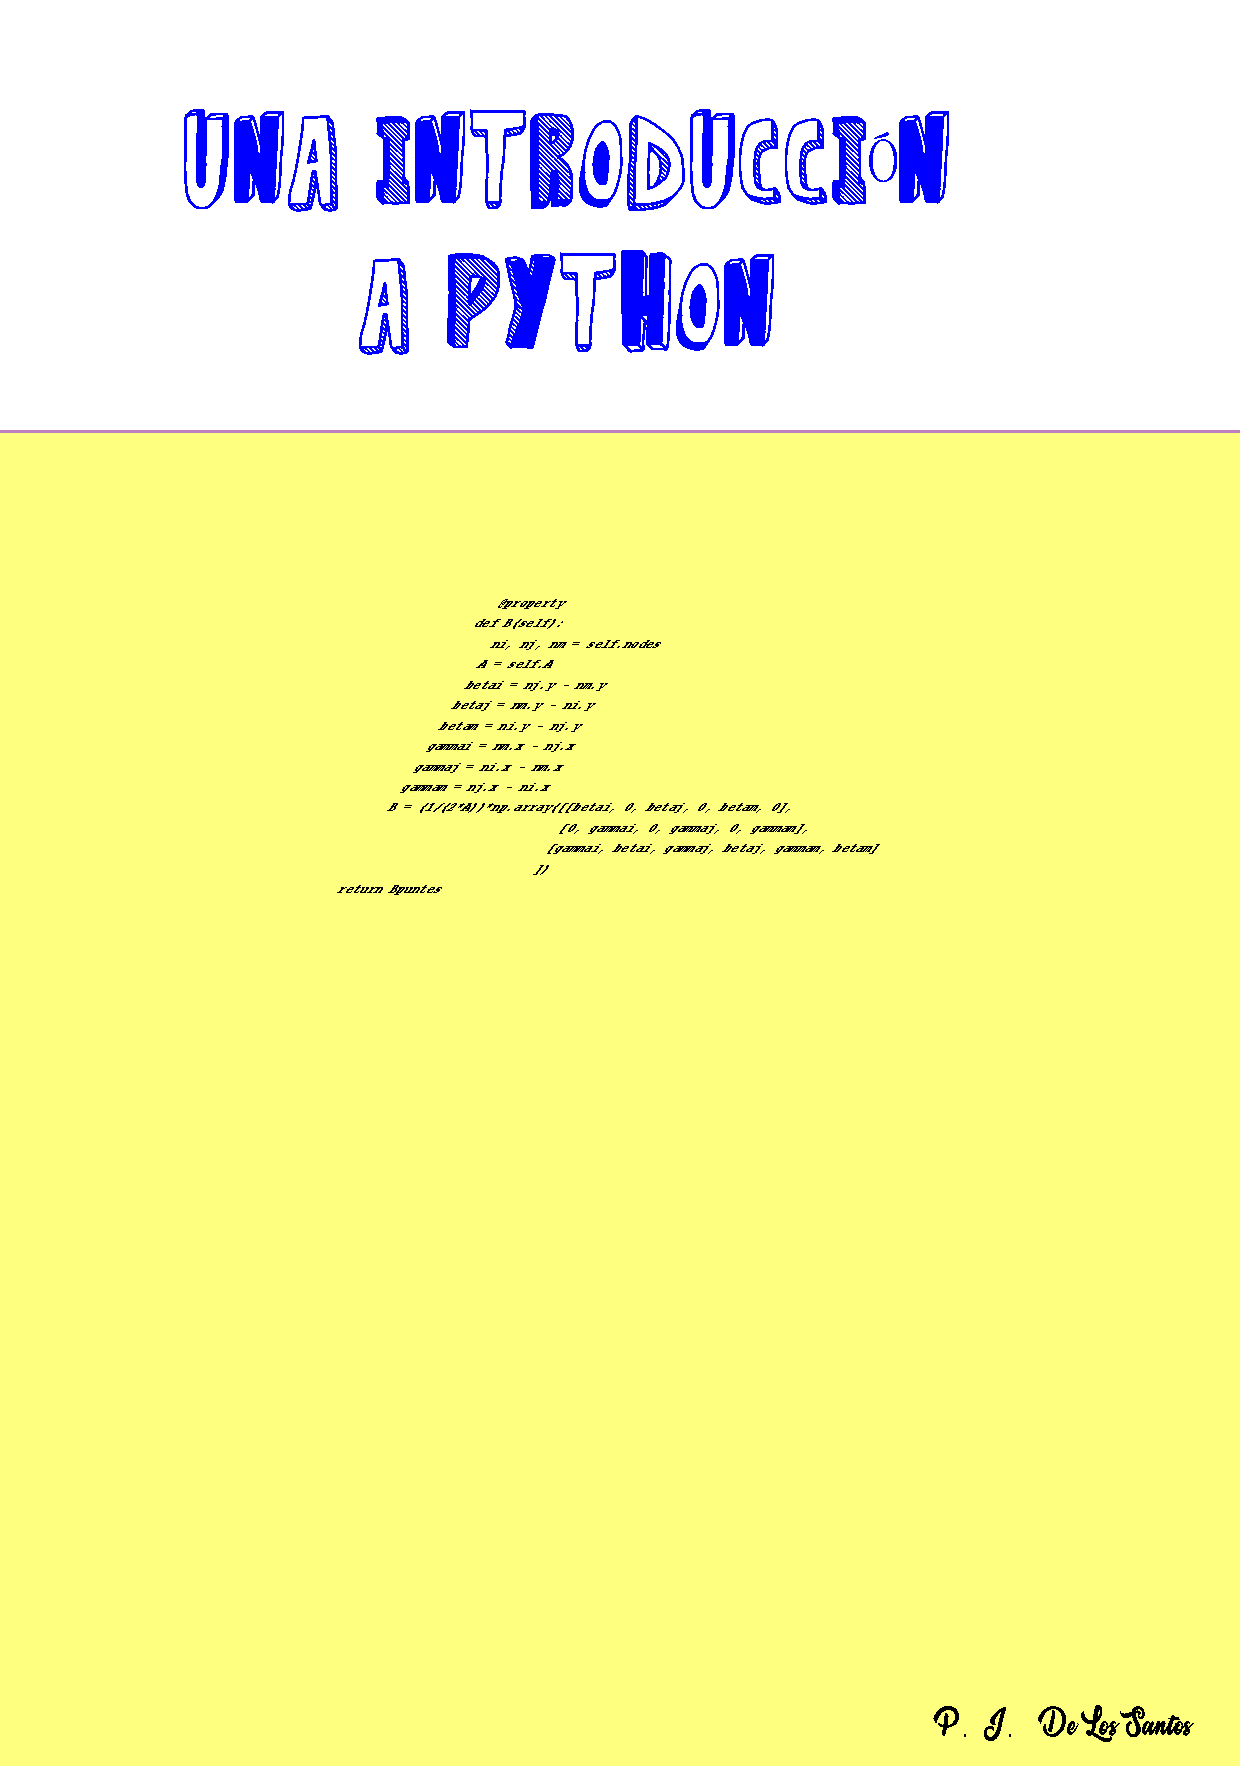
\includepdf[pages=-]{img/cover.pdf}
\maketitle
\tableofcontents


\chapter*{Introducción}
\chapter{Fundamentos del lenguaje}


\section{Python}

Python es un lenguaje de programación, interpretado, de alto nivel y propósito general, además de ser un proyecto  
libre y de código abierto, con una comunidad enorme implicada en el desarrollo y mantenimiento de librerías que hacen 
posible el \textit{multidominio} actual de Python.

Dada su concepción como lenguaje de propósito general, Python es utilizado en una diversidad de aplicaciones, 
desde desarrollo web, encriptación, análisis de datos, procesamiento de imágenes, aprendizaje automático, 
computación simbólica, etc.  

Las características de este lenguaje le hacen propicio para el prototipado de aplicaciones, dado que es muy 
sencillo y rápido revisar y modificar el código desarrollado. Otra característica muy notable de Python 
es su sintaxis simple y fácil de aprender, lo cual ayuda al momento de introducirse en el desarrollo de 
algoritmos o el mundo propio de la programación de computadoras.

\section{Instalando Python}

En estos apuntes se utilizará la distribución Anaconda de Python, la cual contiene el intérprete y las librerías del 
\textit{core}, pero además incluye la mayoría de librerías utilizadas para el desarrollo de aplicaciones de corte 
técnico-científico.

La descarga de Anaconda puede realizarla desde el sitio \url{https://www.anaconda.com/download/}, selecciona el 
paquete de descarga conforme al sistema operativo (Windows, macOS o Linux) así como la arquitectura de su PC.
La instalación suele ser muy sencilla, puede seguir las instrucciones dadas en el \textit{How to install ANACONDA} de 
la misma página.

\section{La consola de Python como una calculadora básica}

Una vez instalado Anaconda puede testear la correcta instalación abriendo \textbf{Anaconda Prompt}, la cual es 
una consola desde la cual puede ejecutar algunos Scripts que complementan el funcionamiento de Python. Puede 
buscar esta consola en la carpeta de instalación correspondiente. Cuando la ejecute observará una consola 
como la mostrada en la figura \ref{fig:anaconda_prompt}

\begin{figure}[h!]
	\centering
	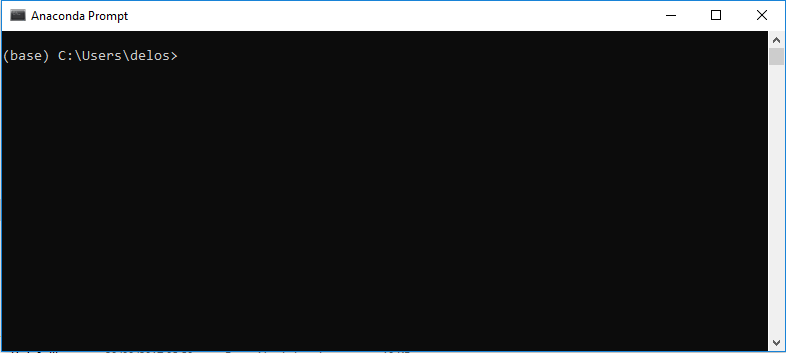
\includegraphics[width=0.75\textwidth]{img/ch01/anaconda_prompt.png}
	\caption{Anaconda Prompt}
	\label{fig:anaconda_prompt}
\end{figure}

Dentro de esta consola escriba \texttt{python} y presione la tecla \textbf{Enter}, al hacer esto observará 
que la consola cambia el prompt compuesto de un directorio por tres signos de \textit{mayor que} tal como 
se puede verificar en la figura \ref{fig:anaconda_prompt_python}.

\begin{figure}[h!]
	\centering
	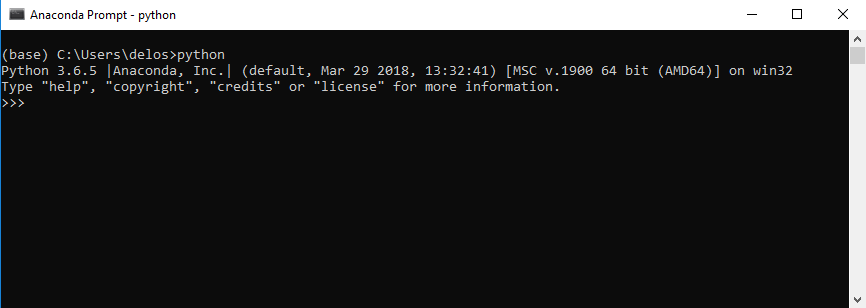
\includegraphics[width=0.75\textwidth]{img/ch01/anaconda_prompt_python.png}
	\caption{Consola Python}
	\label{fig:anaconda_prompt_python}
\end{figure}

A partir de este momento puede ingresar código Python y teclear \textbf{Enter} para ejecutar la instrucción  
y la consola le devolverá lo que resulte de esto. Por ejemplo, si escribe un número cualesquiera y presiona enter, 
la consola le devolverá justamente el mismo número:

\begin{python}
>>> 1000
1000
\end{python}

Puede ejecutar un simple suma aritmética:

\begin{python}
>>> 100 + 200
300
\end{python}

O una resta:

\begin{python}
>>> 550 - 650
-100
\end{python}

Naturalmente Python maneja sin complicaciones las cantidades negativas. Una multiplicación la realiza 
con el operador *:

\begin{python}
>>> 50*25
1250
\end{python}

Para las divisiones utiliza el operador /:

\begin{python}
>>> 1/2
0.5
\end{python}

Puede elevar a una potencia utilizando como operador el doble asterisco:

\begin{python}
>>> 13**2
169
\end{python}

Inclusive existe la posilidad de definir números complejos y realizar operaciones con ellos:

\begin{python}
>>> 5 + 2j
(5+2j)
>>> (5 + 2j) - (10 + 7j)
(-5-5j)
>>> (5 + 2j)*(10 + 7j)
(36+55j)
\end{python}

Puede ampliar la capacidad de las funcionalidades \textit{built-in} de Python si importa alguna librería, como 
\texttt{math}, pero claro, eso será un tema a tratar con posterioridad.

\section{Variables y tipos de datos}

Al ser un lenguaje de alto nivel, Python dispone de los tipos de datos elementales en cualquier lenguaje de programación, 
pero además incluye estructuras de datos muy \textit{avanzadas} y con altas prestaciones que facilitan en muchos 
aspectos la tarea del programador.

Python es un lenguaje de tipado dinámico en el que no hace falta declarar el tipo de dato que asignará a una variable, 
de igual manera una variable puede cambiar de tipo conforme la ejecución del programa, por ello se debe tener cuidado 
con la sintaxis para definir cada tipo de dato.

\subsection{Variables}

Las variables son referencias a los objetos de Python, son creadas por asignación mediante el signo \texttt{=}, 
por ejemplo:

\begin{python}
>>> a = 2
>>> b = 10
>>> a + b
12
\end{python}

El nombre de una variable puede constar de una combinación de caracteres alfanúmericos y el guión bajo, 
siempre y cuando el primer caracter no sea un dígito. Además, en Python los nombres de variables son 
\textit{case sensitive}, es decir, se distingue entre mayúsculas y minúsculas.

\begin{python}
>>> D = 177.8
>>> d = 95
>>> print(D)
177.8
>>> print(d)
95
\end{python}

Existen algunas palabras reservadas del lenguaje que no puede utilizar como nombre de variable, 
puede verificar cuáles son estas palabras tecleando lo siguiente:

\begin{python}
>>> import keyword
>>> keyword.kwlist
['False', 'None', 'True', 'and', 'as', 'assert', 'break', 'class', 'continue', 'def', 'del', 'elif', 'else', 'except', 'finally', 'for', 'from', 'global', 'if', 'import', 'in', 'is', 'lambda', 'nonlocal', 'not', 'or', 'pass', 'raise', 'return', 'try', 'while', 'with', 'yield']
\end{python}


\subsection{Enteros}



\subsection{De coma flotante}



\subsection{Cadenas de caracteres}

Las cadenas de caracteres (denominadas habitualmente y de manera indistinta como \textit{strings}) es un tipo de dato 
que contiene una secuencia de símbolos, mismos que pueden ser alfanúmericos hasta cualquier otro símbolo propio de 
un sistema de escritura. En Python los strings se definen entre comillas dobles o simples:

\begin{python}
>>> "esta es una cadena de caracteres"
'esta es una cadena de caracteres'
>>> 'esta también'
'esta también'
\end{python}

Puede concatenar dos strings utilizando el operador \texttt{+}:

\begin{python}
>>> "Hola" + "mundo"
'Holamundo'
\end{python}

Notará que Python por sí mismo no sabe que estamos uniendo dos palabras y que entre ellas debería haber un espacio 
para su correcta lectura, evidentemente este tipo de cuestiones son las que el programador debe tomar en cuenta al 
escribir un código.

Una cadena de caracteres es lo que en Python se conoce como \textit{iterable}, es decir, una secuencia de 
elementos agrupados a los cuales se puede acceder de manera individual mediante indexación. Por ejemplo, 
sea \texttt{nombre} una cadena de caracteres dada por:

\begin{python}
>>> nombre="Catalina"
\end{python}

Puede acceder a cada una de las letras que componen dicha cadena mediante la notación \texttt{iter[pos]}, donde 
\texttt{iter} es el nombre del iterable y \texttt{pos} la posición en que se encuentra el caracter al cual 
se desea acceder, siendo 0 para la primera letra, 1 para la segunda y así de manera consecutiva. Por ejemplo: 

\begin{python}
>>> nombre[0]
'C'
>>> nombre[4]
'l'
>>> nombre[2]
't'
\end{python}

Al último elemento, sin importar la longitud de la cadena, se accede con el índice -1:

\begin{python}
>>> nombre[-1]
'a'
\end{python}


\subsection{Booleanos}



\subsection{Listas}

Las listas son estructuras de datos que pueden almacenar cualquier otro tipo de dato, inclusive una lista 
puede contener otra lista, además, la cantidad de elementos de una lista se puede modificar removiendo o 
añadiendo elementos. Para definir una lista se utilizan los corchetes, dentro de estos se colocan todos 
los elementos separados por comas:

\begin{python}
>>> calificaciones = [10,9,8,7.5,9]
>>> nombres = ["Ana","Juan","Sofía","Pablo","Tania"]
>>> mezcla = [True, 10.5, "abc", [0,1,1]]
\end{python}

Las listas son iterables y por tanto se puede acceder a sus elementos mediante indexación:

\begin{python}
 >>> nombres[2]
'Sofía'
>>> nombres[-1]
'Tania'
\end{python}

Se tiene la posibilidad de agregar elementos a una lista mediante el método \code{append}: 

\begin{python}
>>> nombres.append("Antonio")
>>> nombres.append("Ximena")
>>> print(nombres)
['Ana', 'Juan', 'Sofía', 'Pablo', 'Tania', 'Antonio', 'Ximena']	
\end{python}

El método \code{remove} elimina un elemento de una lista:

\begin{python}
>>> nombres.remove("Ana")
>>> print(nombres)
['Juan', 'Sofía', 'Pablo', 'Tania', 'Antonio', 'Ximena'] 	
\end{python} 

Sí el valor pasado al método \code{remove} no existe, Python devolverá un \code{ValueError}:

\begin{python}
>>> nombres.remove("Jorge")
Traceback (most recent call last):
  File "<stdin>", line 1, in <module>
ValueError: list.remove(x): x not in list
\end{python}



\subsection{Tuplas}

Las tuplas son secuencias de elementos similares a las listas, la diferencia principal es que 
las tuplas no pueden ser modificadas directamente, es decir, una tupla no dispone de los métodos 
como \code{append} o \code{insert} que modifican los elementos de una lista.

Para definir una tupla, los elementos se separan con comas y se encierran entre paréntesis.

\begin{python}
>>> colores=("Azul","Verde","Rojo","Amarillo","Blanco","Negro","Gris")
\end{python}

Las tuplas al ser \textit{iterables} pueden accederse mediante la notación de corchetes e índice.

\begin{python}
>>> colores[0]
'Azul'
>>> colores[-1]
'Gris'
>>> colores[3]
'Amarillo'
\end{python}

Si intentamos modificar alguno de los elementos de la tupla Python nos devolverá un \code{TypeError}:

\begin{python}
>>> colores[0] = "Café"
Traceback (most recent call last):
  File "<stdin>", line 1, in <module>
TypeError: 'tuple' object does not support item assignment
\end{python}


\subsection{Diccionarios}

Los diccionarios son estructuras que contienen una colección de elementos de la 
forma \textit{clave: valor} separados por comas y encerrados entre llaves. 
Las claves deben ser objetos inmutables y los valores pueden ser de cualquier tipo. 
Necesariamente las claves deben ser únicas en cada diccionario, no así 
los valores. 

Vamos a definir un diccionario llamado \code{edades} en el cual 
cada clave será un nombre y el valor una edad:

\begin{python}
>>> edades = {"Ana": 25, "David": 18, "Lucas": 35, "Ximena": 30, "Ale": 20}
\end{python}

Puede acceder a cada valor de un diccionario mediante su clave, por ejemplo, 
si quisieramos obtener la edad de la clave \code{"Lucas"} se tendría que escribir:

\begin{python}
>>> edades["Lucas"]
35
\end{python}


\section{Operadores relacionales y lógicos}


\section{Control de flujo}

\subsection{Condicional if-elif-else}

El condicional \code{if-elif-else} es una estructura de control que sirve para tomar decisiones 
en el flujo del programa. La sintaxis para \code{if-elif-else} es:

\begin{python}
if cond1:
    # hacer algo 
elif cond2:
    # hacer otra cosa
    .
    .
    .
elif condn:
    # hacer algo más
else:
    # hacer algo por default
\end{python}

Donde \code{cond1, cond2, ... condn} son valores lógicos que resultan de una comparación. Esta estructura se evalúa 
secuencialmente hasta encontrar una condición que se cumpla, si ninguna lo hace, entonces se ejecuta la instrucción 
colocada en el caso por default \code{else}.



\subsection{Bucle for}

El \textbf{bucle for} es una estructura de control de naturaleza repetitiva, en la cual se conocen 
\textit{a priori} el número de iteraciones a realizar \footnote{Aunque no sea tan habitual, un bucle for en Python puede 
romperse mediante instrucciones explícitas de interrupción de ejecución}. 

En lenguajes como C++ o Java, el ciclo for necesita de una variable de ciclo de tipo entero 
que irá incrementándose en cada iteración. En Python, la cuestión es un poco diferente, el ciclo 
for \textit{recorre} un \textit{iterable} y en la k-ésima iteración la variable de ciclo \textit{adopta} el 
valor del elemento en la k-ésima posición del iterable.

De manera general, la sintaxis de for es:

\begin{python}
for var in iterable:
    # Hacer algo ...
\end{python}

Donde \code{var} es la \textbf{variable de ciclo} e \code{iterable} la secuencia de valores que deberá iterarse. 
Es necesario remarcar la importancia de los dos puntos al final de esta primera línea y en indentar el bloque de 
código subsecuente que definirá el cuerpo del ciclo for.

Como primer ejemplo vamos a recorrer una lista de números y mostrarlos por consola:

\begin{python}
numeros = [18,50,90,-20,100,80,37]
for n in numeros:
    print(n)
\end{python}
\begin{outscript}
18
50
90
-20
100
80
37
\end{outscript}

Observe que en cada iteración la variable de ciclo \code{n} adopta el valor de cada uno de los elementos de la 
lista \code{numeros}.

Como ya se mencionó, en Python la variable de ciclo no necesariamente adopta valores numéricos enteros secuenciales, 
si no valores dentro de una secuencia. Esta secuencia podría ser también una cadena de caracteres, por ejemplo:

\begin{python}
palabra = "Python"
for letra in palabra:
    print(letra)
\end{python}
\begin{outscript}
P
y
t
h
o
n
\end{outscript}

Dentro de un ciclo for podemos colocar cualesquiera otra instrucción de control de flujo. Un caso 
muy común es el de incluir otro ciclo for, algo que habitualmente se denota como \textbf{ciclos anidados}. 
Por ejemplo, supongamos que se requieren mostrar por consola todos los elementos de algunas listas contenidas 
dentro de otra lista principal, en ese caso se hace necesario primero iterar sobre la lista principal y 
enseguida hacerlo sobre las listas contenidas, por ejemplo:

\begin{python}
matriz = [[-5,2,0], [9,5,6], [1,7,15]]
for fila in matriz:
    for elemento in fila:
        print(elemento)
\end{python}
\begin{outscript}
-5
2
0
9
5
6
1
7
15
\end{outscript}




\subsection{Bucle while}



\section{Funciones}

Las funciones son \textit{porciones de código} nos sirven para modularizar 
nuestros programas y evitar en muchos casos la repetitividad de código. 
De manera general una función recibe algunos valores de entrada, los \textit{procesa} y 
devuelve algunos valores de salida. 

\subsection{Funciones nativas de Python (\textit{built-in})}

Python dispone de algunas funciones nativas que se \textit{cargan} automáticamente cuando se 
inicia el intérprete. Por ejemplo la función \code{max} devuelve el mayor valor numérico de 
una lista de números:

\begin{python}
>>> max([10,35,5,110,48,30,112,98,87])
112
\end{python}

También existe una función \code{min}, análoga a \code{max}:

\begin{python}
>>> min([10,35,5,110,48,30,112,98,87])
5
\end{python}

Otro ejemplo de función nativa es \code{bin}, la cual dado un número en base 10 devuelve 
una cadena con la representación en base 2.

\begin{python}
>>> bin(10)
'0b1010'
\end{python}

Naturalmente, el valor devuelto por una función se puede asignar a una variable y posteriormente ser utilizado:

\begin{python}
>>> a = max([10,5,8])
>>> b = min([10,5,8])
>>> h = (a - b)/10
>>> print(h)
0.5
\end{python}

Hay funciones como \code{print} que no devuelven como tal un valor, si no que pueden modificar directamente 
alguna variable global o simplemente mostrar algo en la salida estándar como el caso de \code{print}.

Tendremos también funciones que aceptan más de un argumento, por ejemplo a la función \code{round} podemos 
pasarle dos argumentos: un número real y la cantidad de lugares decimales a considerar para el redondeo.

\begin{python}
>>> round(3.141592653589793, 6)
3.141593
>>> round(3.141592653589793, 4)
3.1416
>>> round(3.141592653589793, 2)
3.14
>>> round(3.141592653589793, 0)
3.0
\end{python}



\subsection{Funciones definidas por el usuario}

Además de las funciones nativas de Python, es posible definir nuestras propias funciones. 
En Python, de manera general, una función se define siguiendo la estructura mostrada a continuación:

\begin{python}
def nombre_fun(arg1, arg2, ..., argN):
	# Cuerpo de la función
	# .
	# .
	# .
	return val1, val2, ..., valN
\end{python}

Donde \code{def} es una palabra que debe anteceder siempre a la definición de una función, 
\code{nombre\_fun} es el nombre que se asignará a la función, entre paréntesis y 
separados por comas se colocan los nombres de los argumentos de entrada, los dos puntos 
se colocan después de cerrar el paréntesis e indican que ahí termina el \textit{encabezado} de 
la función y comenzará el \textit{cuerpo} de la misma, aquí se colocarán todas las 
instrucciones que deberán realizarse; la palabra reservada \code{return} sirve para 
indicar los valores a devolver, mismos que se colocarán separados por comas.

Vamos a definir una función llamada \code{saluda}, la cual recibe un nombre (string)
y devuelve un saludo (string) formado mediante concatenación:

\begin{python}
def saluda(nombre):
    s = "Hola " + nombre + ", bienvenido."
    return s

print(saluda("Jorge"))
\end{python}
\begin{outscript}
Hola Jorge, bienvenido.
\end{outscript}

Lo único que hace la función anterior es tomar un \textit{string} como argumento y unirlo 
a algunas cadenas ya establecidas dentro de la función. 

Veamos ahora cómo definir una función que recibe como argumento un entero y devuelve un valor lógico que 
indica si este es par.

\begin{python}
def espar(n):
    if n%2 == 0:
        s = True
    else:
        s = False
    return s

print(espar(2))
print(espar(5))
print(espar(10))
\end{python}
\begin{outscript}
True
False
True
\end{outscript}


Naturalmente, las funciones pueden recibir más de un argumento. Por ejemplo:

\begin{python}
def mayor(a,b):
    m = a
    if a < b:
        m = b
    return m

print( mayor(50,30) )
print( mayor(1100,3050) )
\end{python}
\begin{outscript}
50
3050
\end{outscript}

La función \code{mayor} recibe dos valores numéricos y determina cuál es el mayor de ambos mediante 
una comparación con la sentencia \code{if}. 

¿Pueden las funciones en Python devolver más de un valor? ¡Claro! Hace falta nada más separar 
con comas los valores a devolver.

\begin{python}
def calcula_rectangulo(b,h):
    A = b*h
    P = 2*b + 2*h
    return A, P

print( calcula_rectangulo(10,5) )
print( calcula_rectangulo(50,15) )
\end{python}
\begin{outscript}
(50, 30)
(750, 130)
\end{outscript}

También es posible guardar/asignar los valores devueltos por la función en variables:

\begin{python}
area1, perimetro1 = calcula_rectangulo(100, 20)
print("Área: {0}\nPerímetro: {1}".format(area1, perimetro1))
\end{python}
\begin{outscript}
Área: 2000
Perímetro: 240
\end{outscript}


\subsubsection{Funciones con una cantidad de parámetros indeterminada}

En ocasiones el número de parámetros que deberá recibir una función no puede ser algo fijo. 
Las definiciones de función en Python tienen la flexibilidad de poder recibir una cantidad 
variable de argumentos de entrada. 

Para ejemplificar esto, vamos a crear una función llamada \code{promedio} que calcule 
el promedio de una cierta cantidad de números pasados como argumentos:

\begin{python}
def promedio(*numeros):
    suma = 0
    k = 0
    for n in numeros:
        suma += n
        k += 1
    return suma/k

print(promedio(10,5))
print(promedio(10,50,40,80,20,100))
print(promedio(5,15,10,5))
\end{python}
\begin{outscript}
7.5
50.0
8.75
\end{outscript}

Observe que lo único que hacemos es que al nombre del parámetro le anteponemos un asterisco, esto le indica 
a Python que la cantidad de argumentos de entrada es indeterminada, en principio. Claro está, que el manejo posterior 
de la información es algo que el programador debe tener en cuenta. Dentro del cuerpo de la función 
se debe considerar que el parámetro \code{numeros} será una tupla cuya cantidad de elementos dependerá 
de la cantidad de argumentos ingresados.


\subsubsection{Funciones y los argumentos con nombre}

Una función en Python se puede \textit{mandar a llamar} pasándo los argumentos de manera posicional, es 
decir, en el orden que fueron definidos en la función, o bien, haciendo uso del nombre del parámetro correspondiente 
al argumento que se introduce, por ejemplo:

\begin{python}
def cuenta_cuantas(frase, letra):
    k = 0
    for car in frase:
        if car is letra:
            k += 1
    return k

print( cuenta_cuantas("hola mundo", "o") )
print( cuenta_cuantas(frase="hola mundo", letra="o") )
print( cuenta_cuantas(letra="o", frase="hola mundo") )
\end{python}

La función \code{cuenta\_cuantas} devuelve el número de presencias de una determinada letra en una frase. Observe 
las tres formas en que la \textit{ejecutamos}, todas son equivalentes. En la primera se pasan los argumentos de 
forma posicional, en la segunda y tercera se utilizan los argumentos con nombres, note que en este caso el orden 
en que los argumentos son pasados, es indistinto.

En la definición de funciones es posible también especificar que se pasarán ciertos argumentos con nombre 
sin necesidad de escribirlos de manera explícita. Observe la siguiente función:

\begin{python}
def muestra_puntos(**personas):
    for persona in personas.items():
        print(persona[0] + " tiene " + str(persona[1]) + " puntos")

muestra_puntos(Jorge=8, Paty=10)
print(30*"=")
muestra_puntos(Ana=6, Carlos=9, Victor=4, Daniela=8)
\end{python}
\begin{outscript}
Jorge tiene 8 puntos
Paty tiene 10 puntos
==============================
Ana tiene 6 puntos
Carlos tiene 9 puntos
Victor tiene 4 puntos
Daniela tiene 8 puntos
\end{outscript}

Vea que la definición de la función \code{muestra\_puntos} incluye un parámetro llamado \code{**personas}, esos dos 
asteriscos antes del nombre del parámetro, indican que no se tiene predeterminado el número de argumentos que se 
pasarán, pero además, indica que cada argumento a introducir deberá ser un argumento con nombre.
Dentro del cuerpo de la función el parámetro \code{**personas} es un diccionario cuyas claves 
son los nombres de los argumentos y los valores corresponden a cada valor asignado al argumento.



\section{Ejercicios}


\begin{enumerate}

% \textbf{Estructuras de control}

\item En las siguientes opciones se muestran operaciones aritméticas entre diversos 
objetos de Python. Verifique si es posible realizarlas e indique el resultado, 
de no ser así describa el por qué.

\begin{enumerate}
    \item \code{1 + 2}
    \item \code{1.3 + 2.5}
    \item \verb|"1" + 2|
    \item \verb|"1" + "2"|
    \item \code{[1,2,3] + [10,20]}
    \item \verb|{"a":10, "b":5} + {"h":2, "i":4}|
\end{enumerate}

\item Observe el siguiente código:

\begin{python}
for a,b in [1,2,5,3,8,7]:
    print(a)
\end{python}

Identifique y explique el error.

\item El siguiente código debería imprimir la longitud de cada palabra contenida en la 
lista \code{palabras}. Identifique el error.

\begin{python}
palabras = ["Carro", "Sol", "Mesa", "Dinosaurio", "Girasol", "Silla"]
for palabra in palabras:
    print(len(palabras))
\end{python}

\item Implemente un programa que determine si un número dado es par o impar.

\item Escriba un programa que cuente el número de vocales en una frase. Tome en cuenta que las vocales 
podrían ser tanto mayúsculas como minúsculas.

\item Escriba un programa que aproxime, mediante la suma de Riemann, el área bajo la curva de la función 
$ f(x) = x^2 + 3x $ en el intervalo $ 0 \leq x \leq 10 $. 

\end{enumerate}
\chapter{NumPy: operaciones matriciales}




 \chapter{Matplotlib: visualización gráfica}


\section{Una primera aproximación}

Una de las características de Matplotlib es la facilidad con la que se puede 
comenzar a trazar gráficas, vea el siguiente código:

\begin{python}
import matplotlib.pyplot as plt

plt.plot([5,10,6,-10,15,1])
plt.show()
\end{python}

El código anterior produce la gráfica mostrada en la figura \ref{fig:grafica_01a}. Como puede observar son solamente 
tres líneas de instrucciones, la primera sirve para importar el módulo \code{pyplot} de Matplotlib, el cual contiene 
muchas de las funciones útiles para el trazo de gráficas; la segunda línea ejecuta la función \code{plot} pasando como 
argumento una lista de valores numéricos, y finalmente la tercera línea se encarga de mostrar el elemento gráfico 
resultante en una ventana. 

Se puede obtener un resultado un poco más \textit{trabajado} con unas cuantas líneas más, tal como se 
muestra en la figura \ref{fig:grafica_01b}. Esta gráfica contiene un poco más de información, lo cual es 
deseable para cualquier representación de este tipo.

\begin{python}
import matplotlib.pyplot as plt

plt.plot([0,1,2,3,4,5], [5,10,6,-10,15,1], 'r--o', label="Partícula 1")
plt.xlabel("Tiempo (s)")
plt.ylabel("Posición (m)")
plt.title("Una primera aproximación")
plt.text(2,7,"$ P_1 (2,6) $", color="b")
plt.legend()
plt.grid(ls="--", color="#dadada")
plt.show()
\end{python}


\begin{figure}[h!]
\begin{subfigure}{0.48\textwidth}
\centering
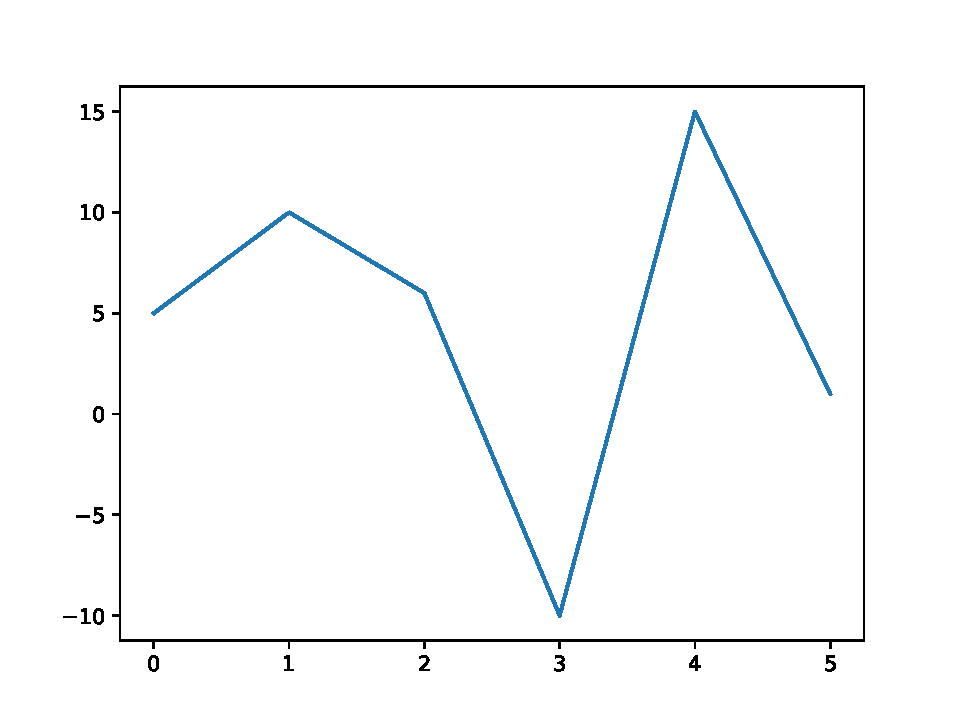
\includegraphics[width=0.9\textwidth]{img/ch03/grafica_01a.pdf}
\captionof{figure}{}
\label{fig:grafica_01a}
\end{subfigure}~
\begin{subfigure}{0.48\textwidth}
\centering
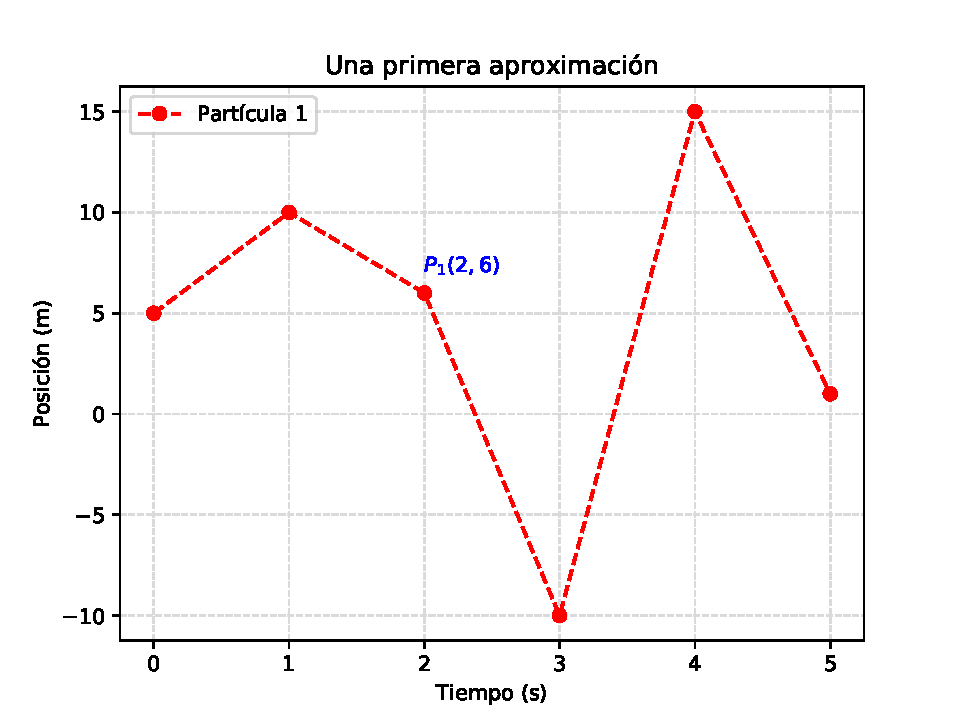
\includegraphics[width=0.9\textwidth]{img/ch03/grafica_01b.pdf}
\captionof{figure}{}
\label{fig:grafica_01b}
\end{subfigure}

\caption{}
\end{figure}



\section{La función \code{plot}}

La función \code{plot} está contenida en el módulo \code{pyplot} y básicamente con esta se produce cualquier gráfica 
bidimensional en coordenadas rectangulares. Esta función soporta varias maneras de ejecutarla dependiendo la cantidad 
de argumentos que se pasen. 

La forma más básica de la función \code{plot} es pasarle un sólo argumento, por ejemplo:

\begin{python}
import matplotlib.pyplot as plt

plt.plot([1,2,3,4,5])
plt.show()
\end{python}

Lo anterior produce una gráfica como la mostrada en la figura \ref{fig:plot_one_argument}. Al pasarle un sólo argumento, 
este se toma como los valores de la coordenada vertical, y se asume que la horizontal varía de 0 a N-1, donde N es el 
número de elementos contenidos en la lista de valores que se introducen.

\begin{figure}[h!]
\centering
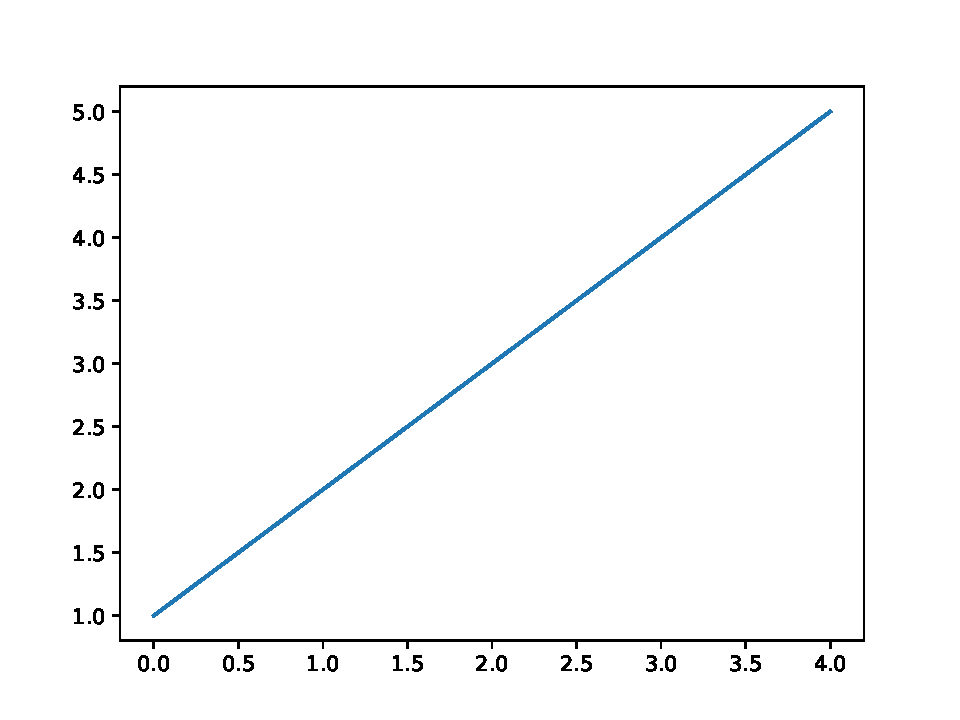
\includegraphics[width=0.55\textwidth]{img/ch03/plot_one_argument.pdf}
\captionof{figure}{}
\label{fig:plot_one_argument}
\end{figure}

La sintaxis más habitual es introducir dos argumentos, donde el primero contiene una lista \code{X} que define los valores 
de la coordenada horizontal, y el segundo una lista \code{Y} correspondiente a los valores de la coordenada vertical, 
por ejemplo:

\begin{python}
import matplotlib.pyplot as plt

plt.plot([10,25,30,60,70,100], [100,200,-100,300,0,-250])
plt.show()
\end{python}

En la figura \ref{fig:plot_two_argument} se muestra la gráfica resultante.

\begin{figure}[h!]
\centering
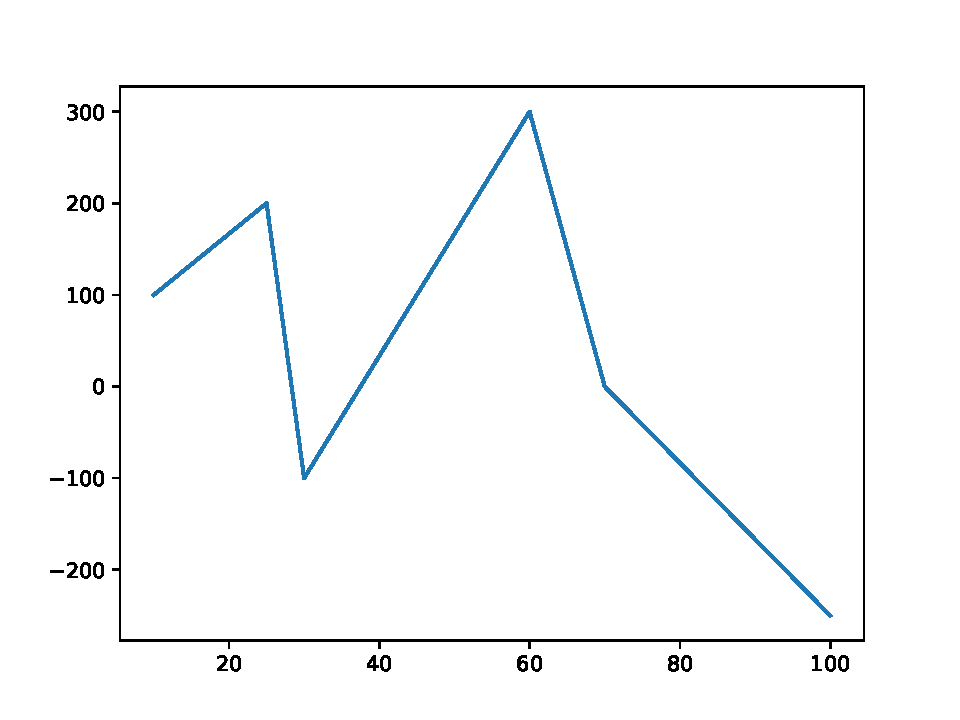
\includegraphics[width=0.55\textwidth]{img/ch03/plot_two_argument.pdf}
\captionof{figure}{}
\label{fig:plot_two_argument}
\end{figure}


\subsection{Graficando funciones matemáticas}

En matemáticas una función es una relación que asigna elementos de un conjunto de manera 
unívoca a otro conjunto. Usualmente una función matemática se puede representar 
mediante una gráfica en coordenadas cartesianas, colocando uno de los conjuntos en el 
eje horizontal y el otro en el vertical.

Utilizando Python, y de manera específica la librería NumPy, se pueden evaluar las funciones 
matemáticas en un intervalo determinado y en una cantidad finita de puntos. 
Por ejemplo, suponga que se requieren calcular todos los pares coordenados correspondientes 
a la función $ y = \cos x $ en el intervalo $ 0 \leq x \leq 5 $, en Python se tendría que definir 
como:

\begin{python}
import numpy as np

x = np.linspace(0,5)
y = np.cos(x)
\end{python}

Las variable \code{x} es un arreglo de NumPy que contiene 50 valores linealmente equiespaciados entre 
0 y 5, la variable \code{y} es también un arreglo de NumPy que resulta de aplicar la función coseno 
a cada valor de \code{x}.

De manera similar a lo anterior se procederá a definir y graficar la función 
$y = e^{-0.1x} \cos x $ en el intervalo $ 0 \leq x \leq 30 $:

\begin{python}
import matplotlib.pyplot as plt
import numpy as np

x = np.linspace(0, 30)
y = np.exp(-0.1*x)*np.cos(x)
plt.plot(x,y)
plt.show()
\end{python}

La gráfica resultante se muestra en la figura \ref{fig:plot_function}. La cantidad de puntos 
a evaluar es una cuestión muy importante, ya que de esto depende la correcta visualización del 
comportamiento de una función. Naturalmente, entre más puntos evaluados mejor será la apreciación 
que se tenga de la curva en cuestión, pero implica un mayor gasto de memoría para guardar y evaluar 
todos los datos. En las figuras \ref{fig:plot_function_more_points} y \ref{fig:plot_function_less_points} 
se muestra la misma función graficada en el mismo intervalo pero con 1000 y 5 puntos evaluados 
de manera respectiva, notará la diferencia entre los tres casos, es evidente que en el caso de los 
5 puntos \textit{se} pierde muchísima información.

\begin{figure}[h!]
\centering
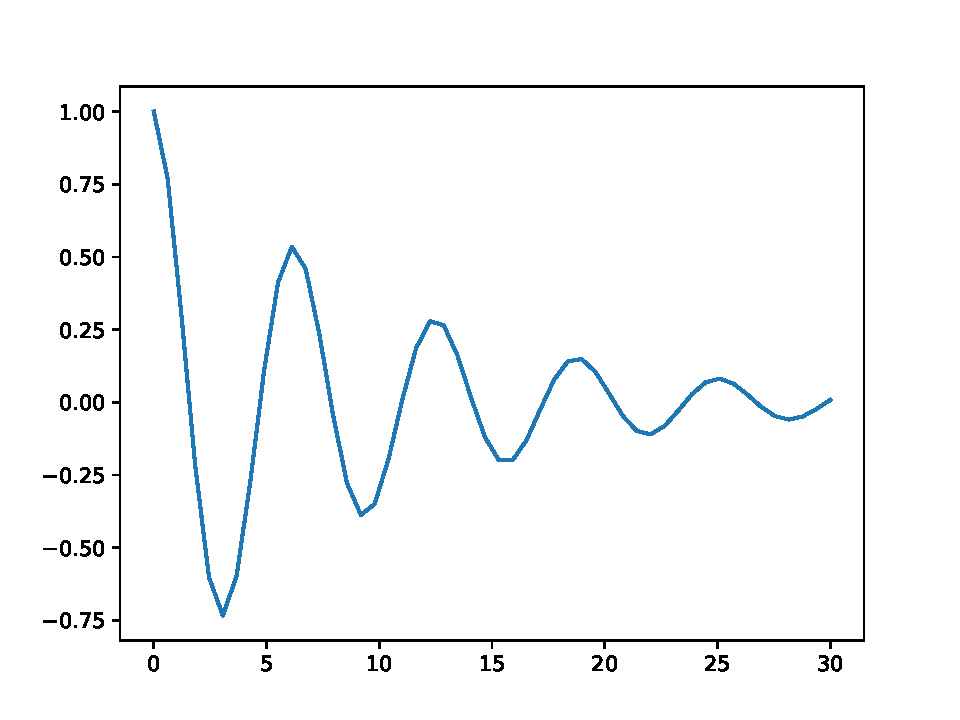
\includegraphics[width=0.55\textwidth]{img/ch03/plot_function.pdf}
\captionof{figure}{}
\label{fig:plot_function}
\end{figure}

\begin{figure}[h!]
\begin{subfigure}{0.48\textwidth}
\centering
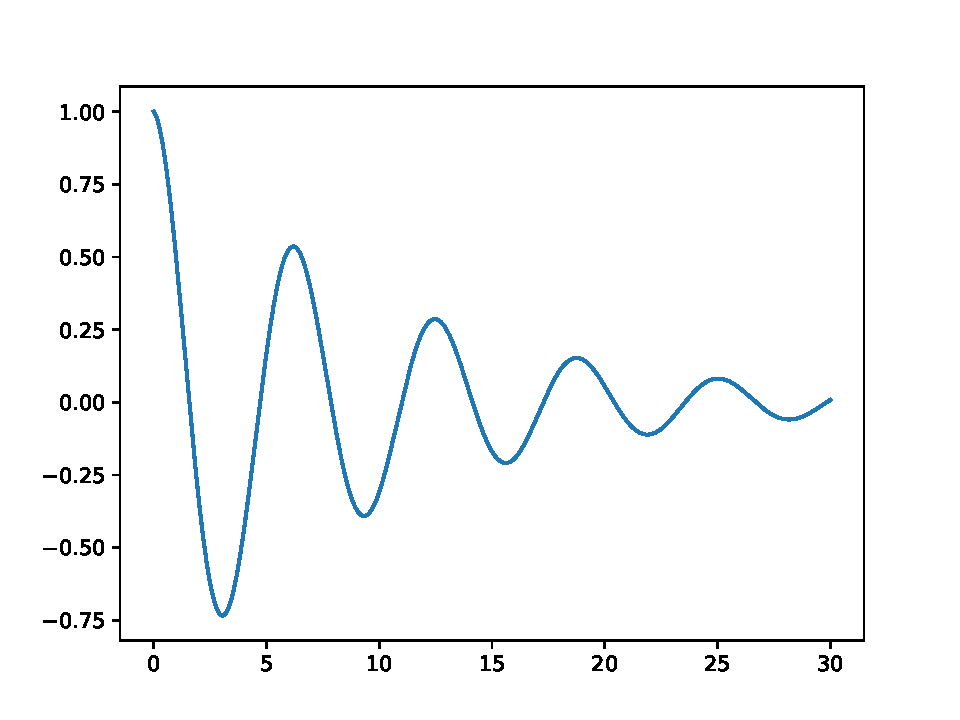
\includegraphics[width=0.9\textwidth]{img/ch03/plot_function_more_points.pdf}
\captionof{figure}{}
\label{fig:plot_function_more_points}
\end{subfigure}~
\begin{subfigure}{0.48\textwidth}
\centering
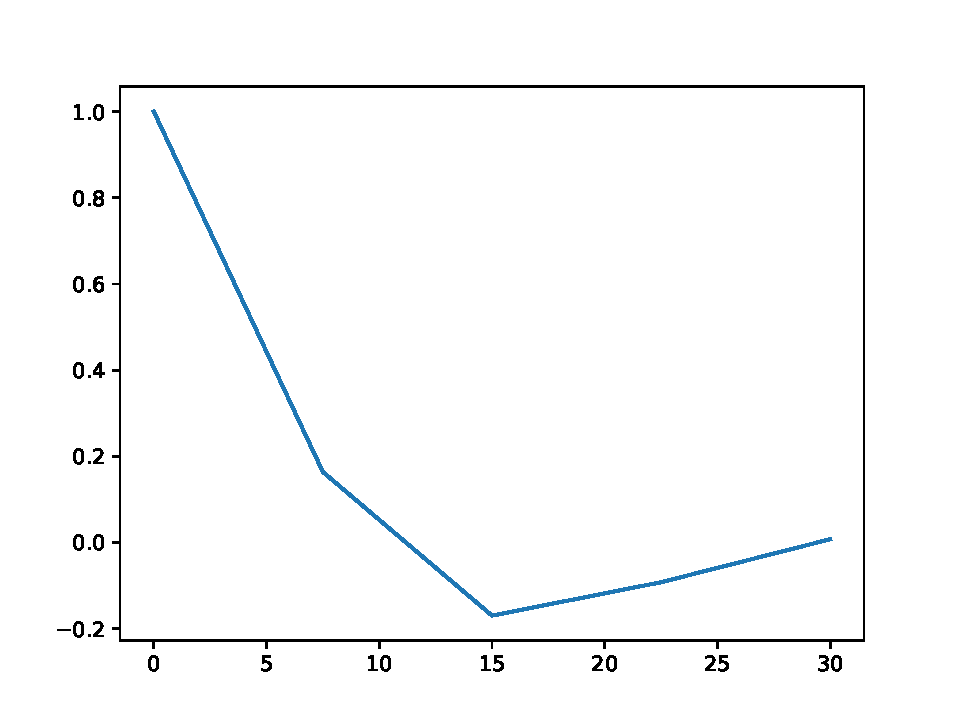
\includegraphics[width=0.9\textwidth]{img/ch03/plot_function_less_points.pdf}
\captionof{figure}{}
\label{fig:plot_function_less_points}
\end{subfigure}

\caption{}
\end{figure}


\subsection{Modificando el color, estilo y grosor de línea}

La función \code{plot} acepta argumentos adicionales que sirven para modificar y controlar características de 
la línea que se grafica. 

Se puede pasar un tercer argumento que contenga una combinación de color y estilo de línea. Por ejemplo:

\begin{python}
import matplotlib.pyplot as plt
import numpy as np

x = np.linspace(0, 30)
y = np.exp(-0.1*x)*np.cos(x)
plt.plot(x, y, "r--")
plt.show()
\end{python}

El código anterior genera una gráfica con una línea en color rojo (\code{r}) y un estilo de línea discontinua 
(\code{-{}-}), tal como se muestra en la figura \ref{fig:plot_color_and_style}. Si en lugar 
del string \code{'r-{}-'} se coloca \code{'go'}, se obtiene una gráfica como la mostrada en la 
figura \ref{fig:plot_color_and_style_02}, podrá inferir que \code{g} refiere al color 
verde (green) y \code{o} justamente al uso de esta como símbolo para representar cada punto.

\begin{figure}[h!]
\begin{subfigure}{0.48\textwidth}
\centering
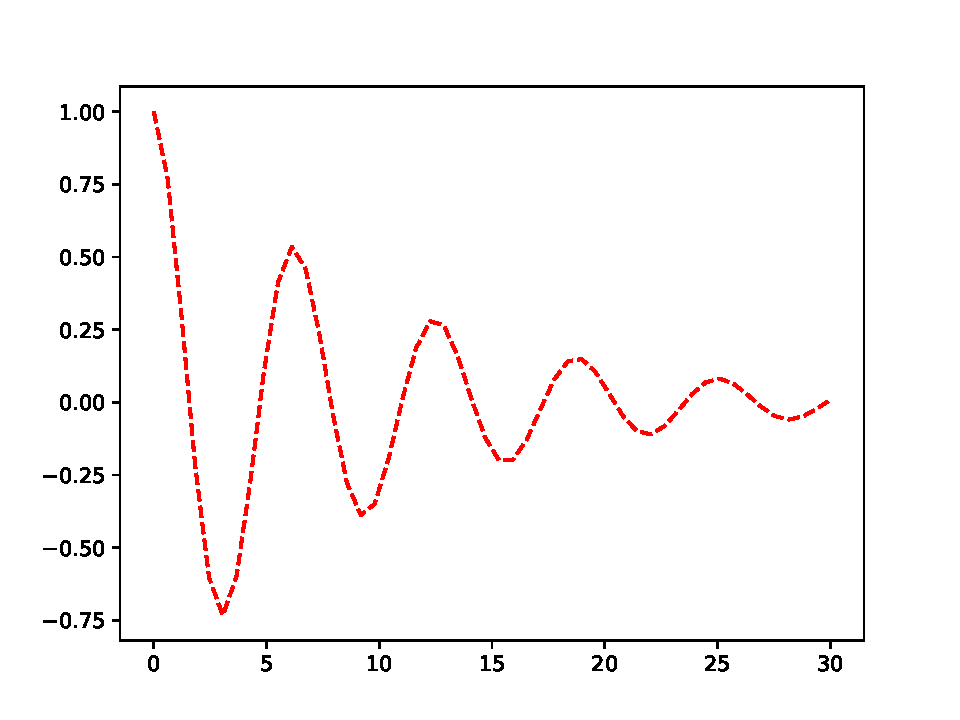
\includegraphics[width=0.9\textwidth]{img/ch03/plot_color_and_style.pdf}
\captionof{figure}{}
\label{fig:plot_color_and_style}
\end{subfigure}~
\begin{subfigure}{0.48\textwidth}
\centering
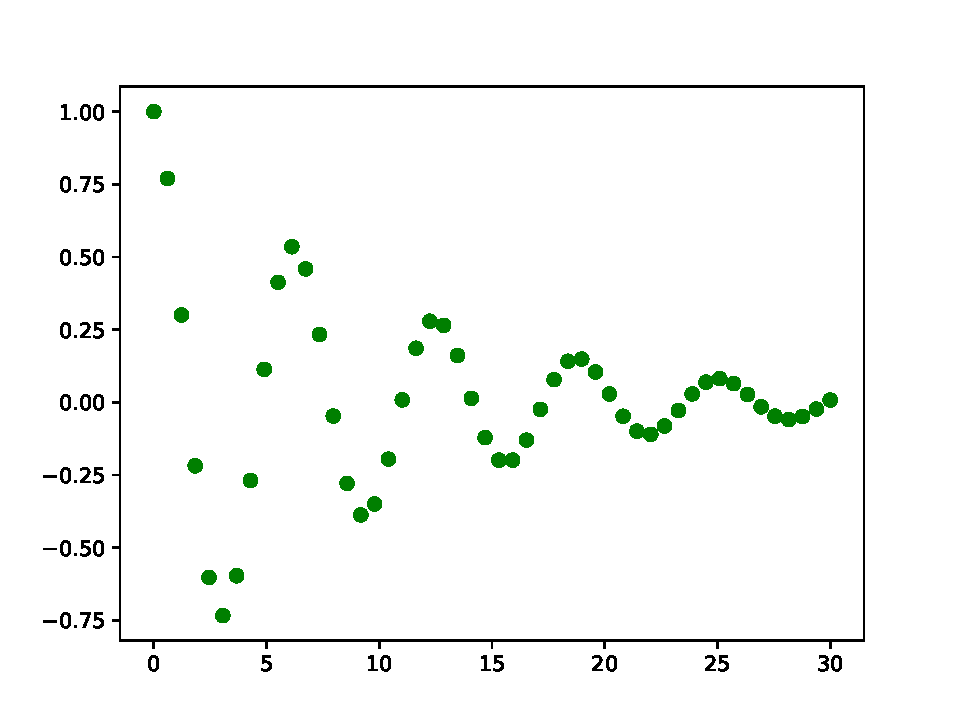
\includegraphics[width=0.9\textwidth]{img/ch03/plot_color_and_style_02.pdf}
\captionof{figure}{}
\label{fig:plot_color_and_style_02}
\end{subfigure}

\caption{}
\end{figure}


En \link{https://matplotlib.org/api/markers_api.html} se muestra una tabla con los símbolos (markers) 
disponibles para utilizar en la función \code{plot}. En \link{https://matplotlib.org/api/colors_api.html} 
puede consultar información respecto a los colores que puede abreviar mediante un sólo caracter.

Además de la forma anterior, también es posible especificar el color y estilo de línea utilizando 
\textit{keyword arguments}, obtendrá el mismo resultado que en la figura \ref{fig:plot_color_and_style} si 
utiliza el siguiente código:

\begin{python}
import matplotlib.pyplot as plt
import numpy as np

x = np.linspace(0, 30)
y = np.exp(-0.1*x)*np.cos(x)
plt.plot(x, y, linestyle="--", color="r")
plt.show()
\end{python}

En ambos casos se especifica un cierto estilo de línea y color, con la diferencia 
notoria de la sintaxis. 

Utilizar \textit{keyword arguments} es una manera más general, puesto que la definición con strings 
no funciona para los casos en que se requieren colores que no se pueden especificar con 
un sólo caracter, por ejemplo, Matplotlib dispone de un color llamado \code{coral} y 
este no puede ser invocado mediante un sólo caracter, hace falta escribir todo el nombre.

El siguiente código produce la gráfica mostrada en la figura \ref{fig:plot_color_and_style_03}, 
note que la clave \code{marker} define el símbolo utilizado para representar cada punto. 

\begin{python}
import matplotlib.pyplot as plt
import numpy as np

x = np.linspace(0, 30)
y = np.exp(-0.1*x)*np.cos(x)
plt.plot(x, y, linestyle="-", color="coral", marker="*")
plt.show()
\end{python}

En la figura \ref{fig:plot_color_and_style_04} se muestra una gráfica bastante similar, 
únicamente difieren en el grosor de la línea, mismo que es controlado con la clave 
\code{linewidth}, del código anterior sólo habría que agregar el argumento \code{linewidth} 
a la función \code{plot}.

\begin{python}
plt.plot(x, y, linestyle="-", color="coral", marker="*", linewidth=3)
\end{python}


\begin{figure}[h!]
\begin{subfigure}{0.48\textwidth}
\centering
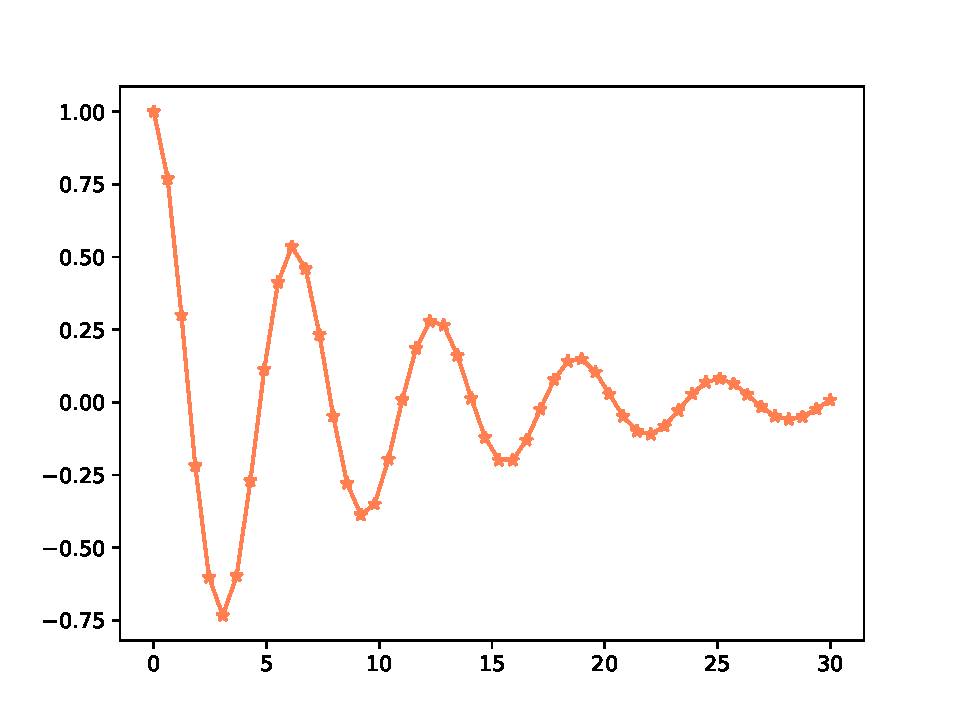
\includegraphics[width=0.99\textwidth]{img/ch03/plot_color_and_style_03.pdf}
\captionof{figure}{}
\label{fig:plot_color_and_style_03}
\end{subfigure}~
\begin{subfigure}{0.48\textwidth}
\centering
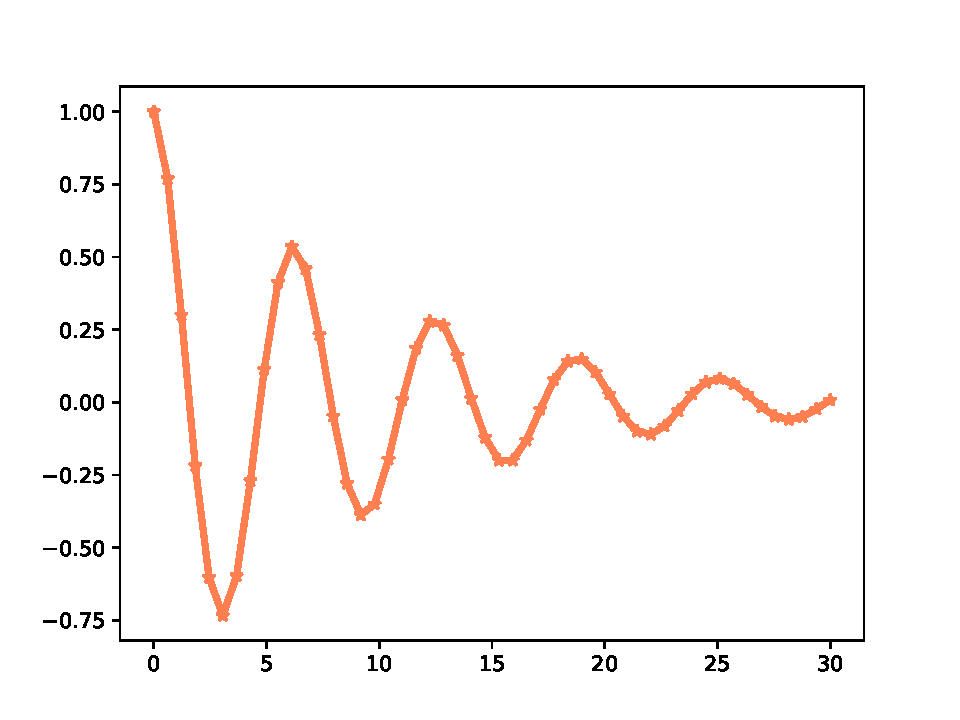
\includegraphics[width=0.99\textwidth]{img/ch03/plot_color_and_style_04.pdf}
\captionof{figure}{}
\label{fig:plot_color_and_style_04}
\end{subfigure}

\caption{}
\end{figure}

\subsection{Título de gráfica, etiquetas de ejes y nombres de curvas}

Por su naturaleza las gráficas nos sirven para presentar y/o visualizar información de ciertos datos, para 
lo cual se hace necesario especificar información descriptiva de lo que se muestra. Es muy común 
que se agreguen etiquetas a los ejes horizontal y vertical, así como el nombre de gráfica. Además, si 
se está graficando más de una curva, se hace necesario especificar a que refiere cada una de ellas.

El siguiente código produce la gráfica mostrada en la figura \ref{fig:plot_xlabel_ylabel_title}. 

\begin{python}
import matplotlib.pyplot as plt
import numpy as np

x = np.linspace(0, 30, 500)
y1 = np.exp(-0.1*x)*np.cos(x)
y2 = np.exp(-0.2*x)*np.sin(x)
plt.plot(x, y1, "b-", label="Partícula 1")
plt.plot(x, y2, "r-", label="Partícula 2")
plt.xlabel("Tiempo (s)")
plt.ylabel("Posición (mm)")
plt.title("Gráfica de posición")
plt.legend()
plt.show()
\end{python}

La instrucción \code{xlabel} coloca una etiqueta al eje horizontal, de manera similar \code{ylabel} lo hace para el eje 
vertical. Con \code{title} adicionamos un título a la gráfica. La instrucción \code{legend} sirve para 
colocar el recuadro con \textit{nombre} asignado a cada curva mediante el \textit{keyword argument} \code{label}.

\begin{figure}[H]
	\centering
	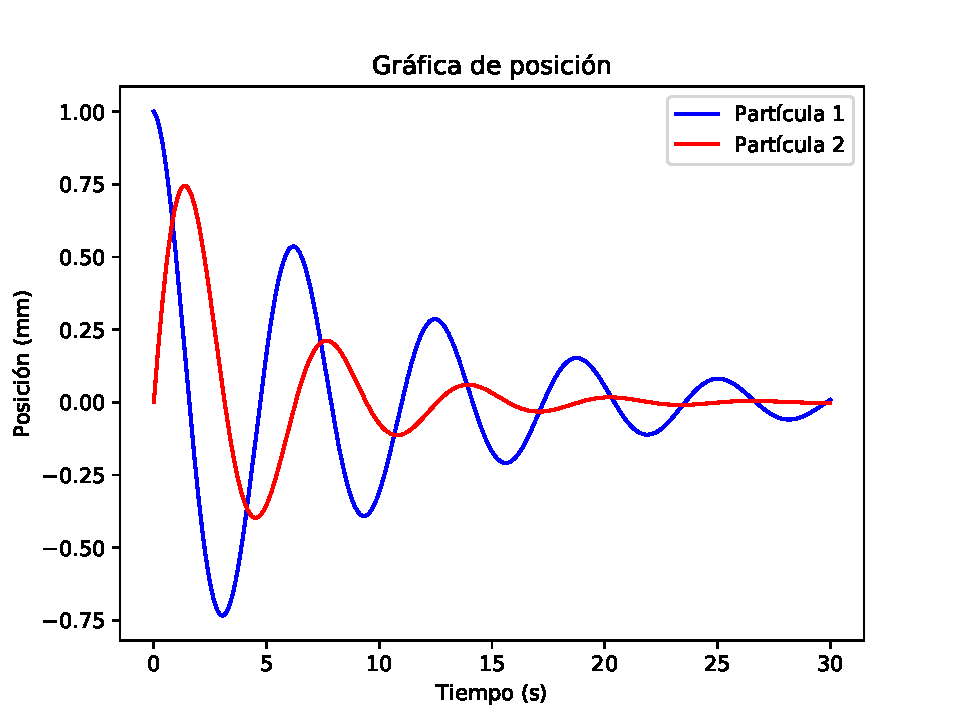
\includegraphics[width=0.55\textwidth]{img/ch03/plot_xlabel_ylabel_title.pdf}
	\caption{}
	\label{fig:plot_xlabel_ylabel_title}
\end{figure}

\subsection{Anotaciones}

Con anotaciones nos referimos a cualesquiera texto que se coloque dentro del \textit{Axes} de Matplotlib. Usualmente 
utilizadas para indicar ciertas características partículares en una gráfica, o bien alguna nota informativa al respecto.
La función base para realizar este tipo de tareas es \code{text}. La sintaxis más simple de \code{text} es:

\begin{python}
plt.text(px, py, texto)
\end{python}

Donde \code{px} y \code{py} denotan las coordenadas en donde se colocará la anotación indicado en \code{texto}. 
Veamos un ejemplo:

\begin{python}
import matplotlib.pyplot as plt
import numpy as np

x = np.linspace(0, 30, 200)
y = np.exp(-0.1*x)*np.cos(x)
plt.plot(x, y, "m")
plt.xlabel("Tiempo (s)")
plt.ylabel("Posición (mm)")
plt.title("Gráfica de posición")
plt.text(10, 0.5, "Algo informativo")
plt.show()
\end{python}

El código anterior produce la gráfica mostrada en la figura \ref{fig:plot_text}. Note que únicamente colocamos 
el texto \textit{Algo informativo}  dentro del gráfico, de manera más específica en las coordenadas (10,0.5).

\begin{figure}[H]
	\centering
	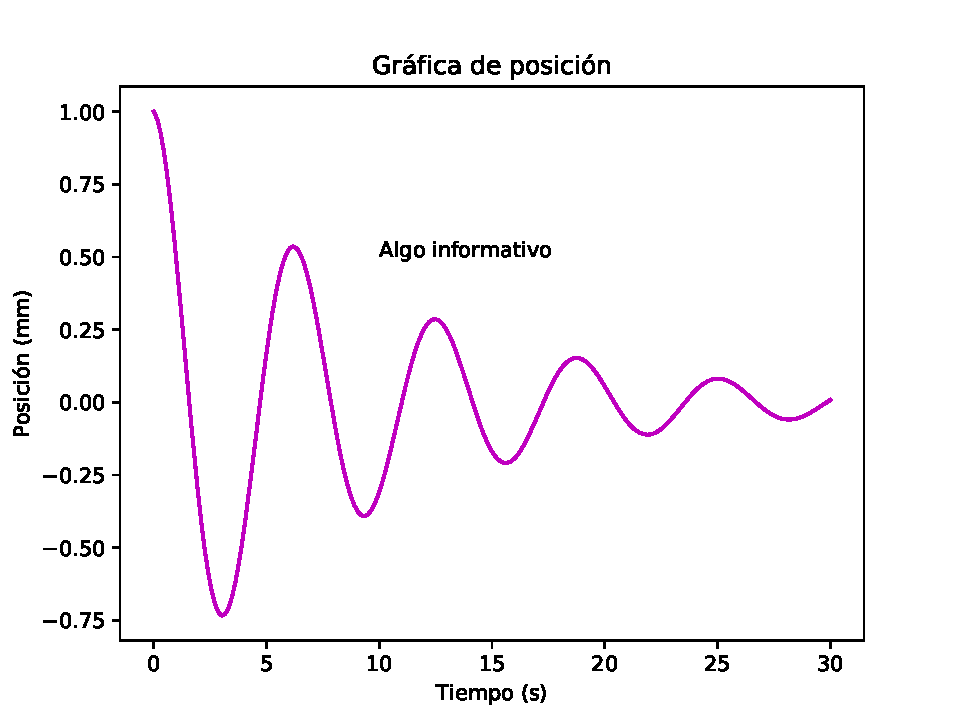
\includegraphics[width=0.55\textwidth]{img/ch03/plot_text.pdf}
	\caption{}
	\label{fig:plot_text}
\end{figure}

Al texto colocado podemos darle formato y ajustarlo a nuestros requerimientos, para ello a la función 
\code{text} se le pueden incluir los \textit{keyword arguments} descritos en \link{https://matplotlib.org/users/text_props.html}. 
Por ejemplo:

\begin{python}
import matplotlib.pyplot as plt
import numpy as np

x = np.linspace(0, 30, 200)
y = np.exp(-0.1*x)*np.cos(x)
plt.plot(x, y, "m")
plt.xlabel("Tiempo (s)")
plt.ylabel("Posición (mm)")
plt.title("Gráfica de posición")
plt.text(10, 0.5, "Algo informativo", fontsize=16, color="r", 
         name="Courier New")
plt.show()
\end{python}

Este código produce la gráfica mostrada en \ref{fig:plot_text_2}, observe que lo único que se cambió fueron algunas 
propiedades del texto, tales como el tamaño de la fuente con \code{fontsize}, el color de fuente con \code{color} 
y el tipo de fuente con \code{name}, con este último se debe tener cuidado, dado que el nombre de la fuente indicada 
debe estar instalada en la PC que se ejecuta. 

\begin{figure}[H]
	\centering
	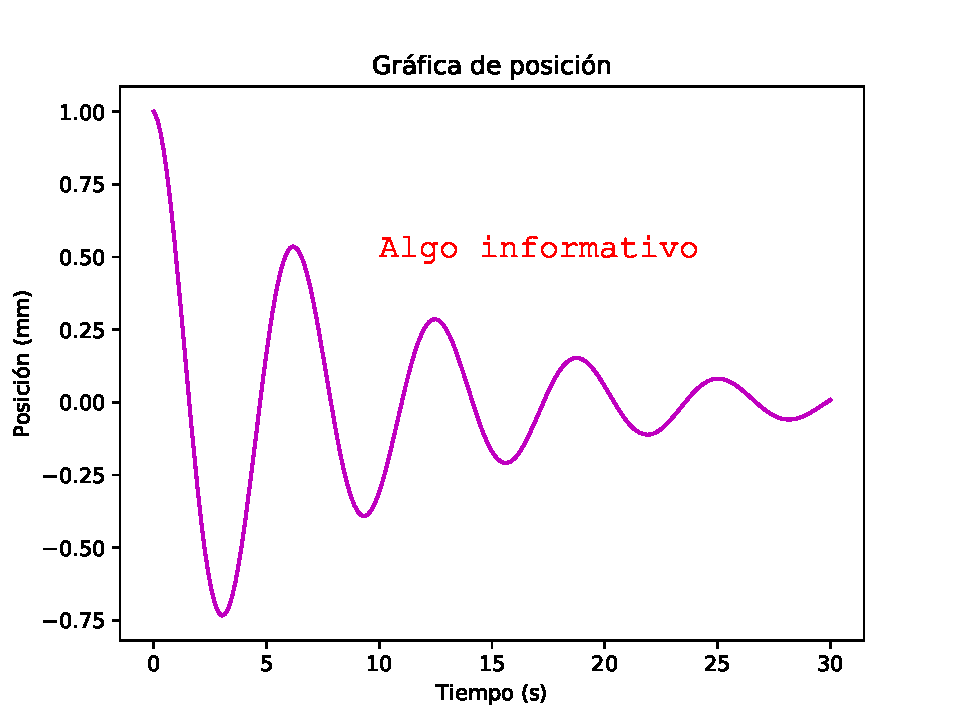
\includegraphics[width=0.55\textwidth]{img/ch03/plot_text_2.pdf}
	\caption{}
	\label{fig:plot_text_2}
\end{figure}


\section{Gráficas en coordenadas polares}

Las coordenadas polares o sistema de coordenadas polares son un sistema de coordenadas bidimensional en el que cada punto del plano se determina por una distancia y un ángulo \footnote{Tomado de: https://es.wikipedia.org/wiki/Coordenadas\_polares}. Habitualmente 
las funciones en coordenadas polares tienen la forma $ r = f(\theta)$.

En Matplotlib se dispone de la función \code{polar}, la cual traza una gráfica en coordenadas polares, dados como argumentos 
tanto la variable independiente $\theta$ como la función $r$. Enseguida vamos a ver cómo graficar la tan conocida 
\textbf{rosa polar}, cuya ecuación general está dada por:

$$ r = a \cos\left( k\theta + \phi_0 \right) $$

Implementando esto en Python, se tiene:

\begin{python}
import matplotlib.pyplot as plt
import numpy as np

theta = np.linspace(0, 2*np.pi, 1000)
a,k,phi0 = 5,7,0
r = a*np.cos(k*theta + phi0)
plt.polar(theta, r, "r")
plt.show()
\end{python}

El código anterior produce la gráfica mostrada en \ref{fig:polar_01}. Observe que la función \code{polar} 
funciona de manera bastante similar a \code{plot}, de hecho se le pueden pasar los mismos 
\textit{keyword arguments} para personalizar el gráfico resultante.

\begin{figure}[H]
	\centering
	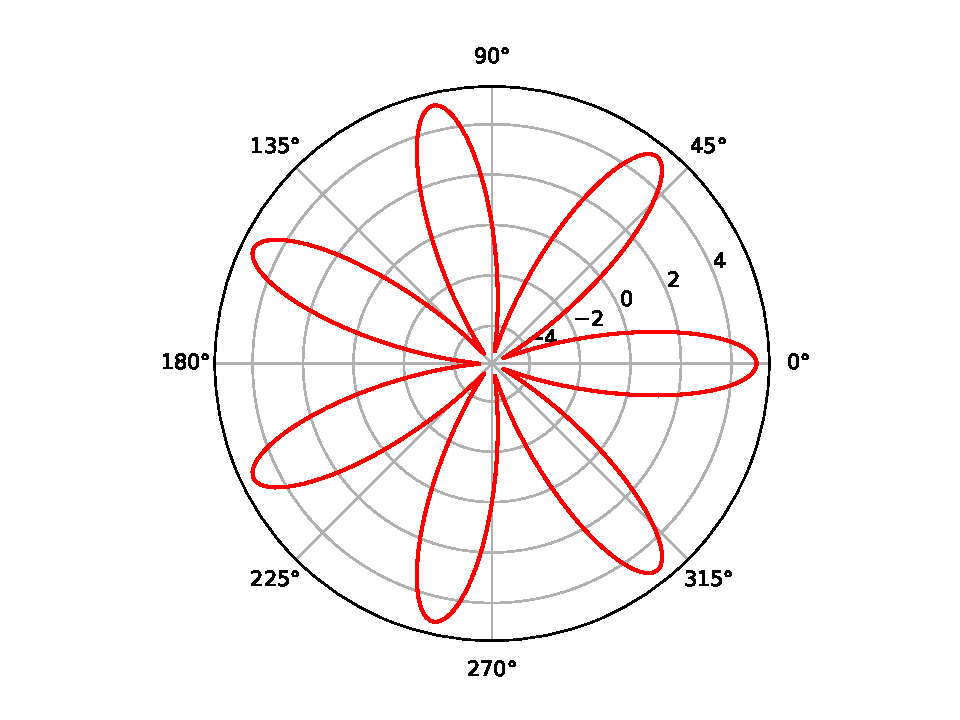
\includegraphics[width=0.55\textwidth]{img/ch03/polar_01.pdf}
	\caption{}
	\label{fig:polar_01}
\end{figure}


\section{Gráficas de barras}



\section{Gráficas de curvas paramétricas en el espacio}

Una función vectorial de la forma: 

$$ \vec{r}(t) = \begin{bmatrix}
x(t) \\ y(t) \\ z(t)
\end{bmatrix} $$

Se dice que es una función parámetrica, siendo $t$ en este caso el parámetro correspondiente. Una función vectorial 
de este tipo tiene una curva en el espacio asociada como representación gráfica. Es muy común 
trabajar con este tipo de expresiones en el análisis cinemático de partículas.

Supongamos que queremos graficar la función vectorial:

$$ \vec{r}(t) = \begin{bmatrix}
\cos(t) \\ \sin(t) \\ t	
\end{bmatrix} $$

En el intervalo $ 0 \leq t \leq 4\pi $. Para ello en Python haríamos lo siguiente:

\begin{python}
from mpl_toolkits.mplot3d import Axes3D
import matplotlib.pyplot as plt
import numpy as np

fig = plt.figure()
ax = fig.add_subplot(111, projection="3d")

t = np.linspace(0, 4*np.pi, 100)
x = np.cos(t)
y = np.sin(t)
z = t

ax.plot(x, y, z)
plt.show()
\end{python}

En la figura \ref{fig:parametric_curve_01} se muestra la gráfica producida. Ahora explicamos lo referente al código 
anterior. Observe que en la primera línea importamos la clase \code{Axes3D} del módulo \code{mpl\_toolkits.maplot3d}, 
esto nos sirve para poder trabajar con gráficas tridimensionales. Luego, definimos un objeto de la 
clase \code{Figure} y lo asignamos a la variable \code{fig}, al objeto \code{fig} le añadimos un 
\textit{Axes} mediante el método \code{add\_subplot}, indicando que dicho \textit{axes} se utilizarán las 
proyecciones espaciales mediante el \textit{keyword argument} \code{projection}. Las siguientes cuatro líneas 
definen las ecuaciones parámetricas. Y, finalmente con el método \code{plot} del objeto \code{ax} trazamos la 
gráfica de la curva tridimensional, note que en este caso el método \code{plot}, recibe al menos tres argumentos: 
las coordenadas en x, y, z.

\begin{figure}[H]
\begin{subfigure}{0.48\textwidth}
\centering
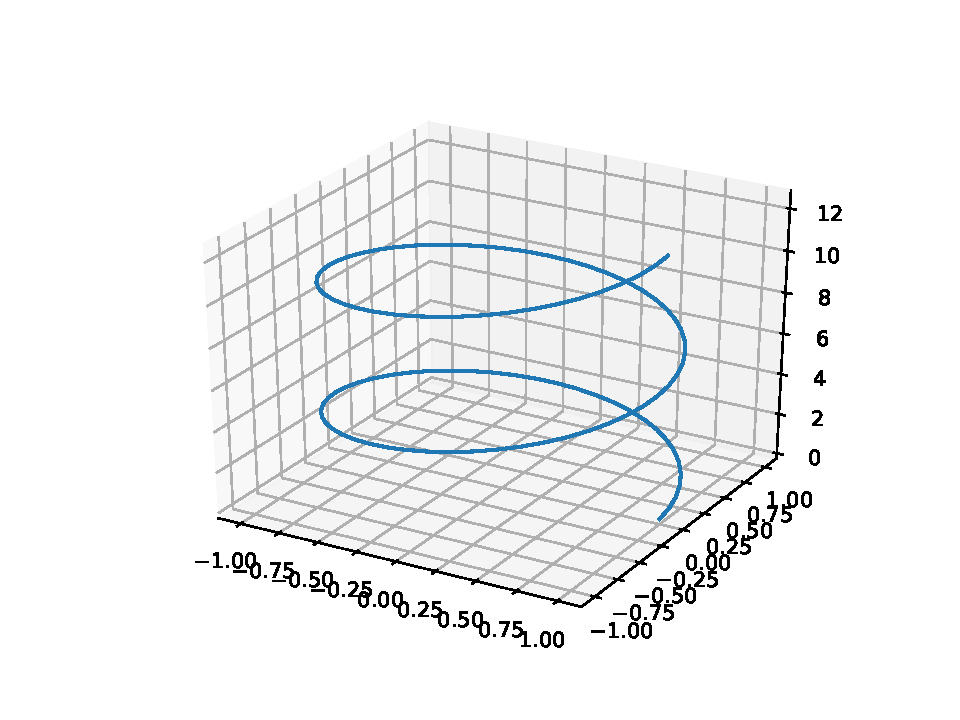
\includegraphics[width=0.9\textwidth]{img/ch03/parametric_curve_01.pdf}
\captionof{figure}{}
\label{fig:parametric_curve_01}
\end{subfigure}~
\begin{subfigure}{0.48\textwidth}
\centering
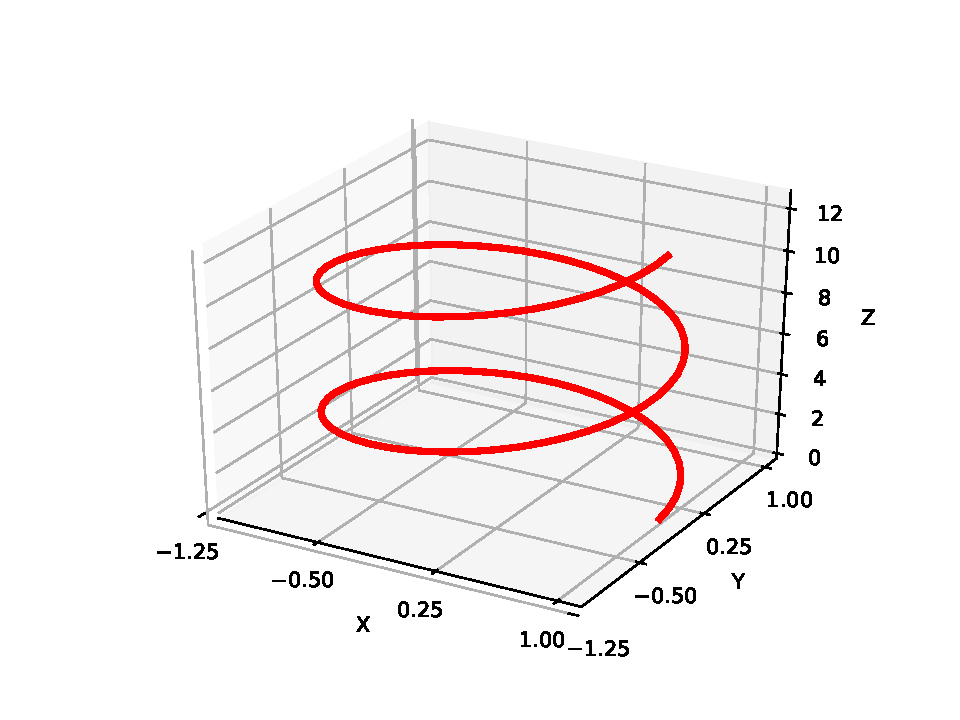
\includegraphics[width=0.9\textwidth]{img/ch03/parametric_curve_02.pdf}
\captionof{figure}{}
\label{fig:parametric_curve_02}
\end{subfigure}

\caption{}
\end{figure}

Al igual que en las otros tipos de gráficos, podemos también manipular las características. Vea por 
ejemplo el siguiente código:

\begin{python}
from mpl_toolkits.mplot3d import Axes3D
import matplotlib.pyplot as plt
import numpy as np

fig = plt.figure()
ax = fig.add_subplot(111, projection="3d")

t = np.linspace(0, 4*np.pi, 100)
x = np.cos(t)
y = np.sin(t)
z = t

ax.plot(x, y, z, color="r", linewidth=3)
xticks = ax.get_xticks()
yticks = ax.get_yticks()
ax.set_xticks(xticks[::3])
ax.set_yticks(yticks[::3])
ax.set_xlabel("X")
ax.set_ylabel("Y")
ax.set_zlabel("Z")
plt.show()
\end{python}

La gráfica producida se muestra en la figura \ref{fig:parametric_curve_02}.


\section{Gráficas de superficies}


\section{Ejercicios}

\begin{enumerate}
\item Grafique las siguientes funciones en el intervalo indicado:
\begin{enumerate}
\item $ y = \cos x + x \qquad 0 \leq x \leq 6\pi $ 
\item $ x = t^2 - 3t \qquad -10 \leq t \leq 10 $ 
\end{enumerate}

\end{enumerate}
\chapter{SymPy: un sistema de álgebra computacional}

SymPy es un sistema de álgebra computacional (CAS) escrito en Python puro, está desarrollado con un enfoque 
en la extensibilidad y facilidad de uso, tanto a través de aplicaciones interactivas como programáticas. Estas 
características le han permitido a SymPy convertirse en una librería de cómputo simbólico muy popular en 
el ecosistema científico de Python. \cite{sympy2017}

En todo el capítulo se asumirá que se ha importado la librería SymPy, con las siguientes instrucciones:

\begin{python}
>>> from sympy import *
\end{python}

\section{Variables simbólicas}

Las variables simbólicas son el \textit{alma} de SymPy, todas las operaciones de álgebra simbólica se basan en estas. 
A una variable simbólica se le asigna un símbolo que la representa mediante la función \code{symbols}:

\begin{python}
>>> x = symbols("x")
>>> print(type(x))
<class 'sympy.core.symbol.Symbol'>
\end{python}

Con la función \code{symbols} se define una nueva variable simbólica que se guarda en \code{x}, se verifica 
que se crea un objeto de la clase \code{Symbol}. Con la variable \code{x} ya definida se puede comenzar 
a formar expresiones algebraicas y manipular matemáticamente.

\begin{python}
>>> x + 2
x + 2
>>> x**2 - 2*x - 10
x**2 - 2*x - 10
>>> sqrt(x) - sin(x)
sqrt(x) - sin(x)
\end{python}

Puede definir múltiples variables separando por comas cada representación simbólica:

\begin{python}
>>> p,q,r = symbols("p,q,r")
>>> p**q + r/q
p**q + r/q
\end{python}

Además de la forma anterior, también es posible tener variables simbólicas disponibles si se importan 
del módulo \code{abc} de SymPy:

\begin{python}
>>> from sympy.abc import a,b,c,d
>>> (a + b)*(c + d)
(a + b)*(c + d)
\end{python}


\section{Manipulación algebraica}

SymPy es una poderosa herramienta de manipulación y simplificación algebraica, en lo subsiguiente se revisarán 
algunos casos elementales y se describirá el uso de las herramientas (funciones) que proporciona.

En primera instancia se definen algunas variables simbólicas a utilizar:

\begin{python}
>>> x,y,z = symbols("x,y,z")
>>> a,b,c,d,k,m,n = symbols("a,b,c,d,k,m,n")
\end{python}

Para las expresiones algebraicas formadas en SymPy por default se \textit{evalúan} y simplifican los términos semejantes. 
Vea los siguientes casos:

\begin{python}
>>> x**2 + 5*x**3 - 10*x**2 + 5*x - 10*(x + 1)
5*x**3 - 9*x**2 - 5*x - 10
>>> a*b + c*d + x/y - 7*a*b
-6*a*b + c*d + x/y
\end{python}

Naturalmente para simplificaciones y operaciones un poco menos obvias, habrá que especificarle lo que se requiere.

Una de las operaciones elementales de simplificación en álgebra es la factorización, SymPy dispone de la 
función \code{factor}, la cual toma una expresión algebraica y la factoriza conforme sea posible. 
Por ejemplo, suponiendo que se tiene la expresión $ab + ac$, es sencillo identificar que se puede  
factorizar como $a(b+c)$, SymPy hace lo mismo sin sobresalto alguno.

\begin{python}
>>> factor(a*b + a*c)
a*(b + c)
\end{python}

De igual forma se sabe que una expresión de la forma $ ac + ad + bc + bd $ se puede factorizar como 
$ (a + b) (d + c) $.

\begin{python}
>>> factor( a*c + a*d + b*c + b*d )
(a + b)*(c + d)
\end{python}

Así, para un binomio al cuadrado se sabe que, $ (a+b)(a+b) $ es la factorización de una expresión del tipo
$ a^2 + 2ab + b^2 $.

\begin{python}
>>> factor(a**2 + 2*a*b + b**2)
(a + b)**2
\end{python}

% \begin{python}
% >>> factor( x**2 - 10*x + 21 )
% (x - 7)*(x - 3)
% \end{python}

¿Se puede hacer el proceso \textit{inverso}, es decir, dados dos factores obtener su expresión \textit{expandida}? 
Por supuesto, para ello se hace uso de la función \code{expand}. 

\begin{python}
>>> expand( (x-7)*(x-3) )
x**2 - 10*x + 21
\end{python}

SymPy puede manejar cualquier cantidad de factores y devolver la expresión que resulta de realizar la multiplicación 
algebraica, sin estar limitada siquiera por la cantidad de variables simbólicas.

\begin{python}
>>> expand( (x + y)*(x - y) )
x**2 - y**2
>>> expand( (x + y)*(x+y) )
x**2 + 2*x*y + y**2
>>> expand( (x + y)**2 )
x**2 + 2*x*y + y**2
>>> expand( (x + y)**3 )
x**3 + 3*x**2*y + 3*x*y**2 + y**3
>>> expand( a*(m + n)**2 )
a*m**2 + 2*a*m*n + a*n**2
\end{python}

De manera general, si requiere simplificar una expresión algebraica SymPy dispone de una función más o menos universal que funcionará en la mayoría de los casos: \code{simplify}. Por ejemplo, suponiendo que 
se tiene la siguiente expresión algebraica racional y se requiere reducir lo más posible:

$$ \frac{x^2 - 3x}{x^2 + 3x}$$

Se puede notar que tanto en el numerador como en el denominador se puede factorizar $x$, lo cual conduce a:

$$ \frac{x(x - 3)}{x(x + 3)} = \frac{x-3}{x+3} $$

Con SymPy:

\begin{python}
>>> simplify( (x**2 - 3*x)/(x**2 + 3*x) )
(x - 3)/(x + 3)
\end{python}

Lo mismo para una expresión que involucre funciones trigonométricas, por ejemplo, cualquiera que haya cursado matemáticas 
del nivel secundario, al menos, sabe que $\sin^2 x + \cos^2 x = 1 $, y también \textit{lo sabe} SymPy:

\begin{python}
>>> simplify( sin(x)**2 + cos(x)**2 )
1
\end{python}

Pero también \textit{sabe} que $ \cos x \cos y - \sin x \sin y = \cos(x+y) $.

\begin{python}
>>> simplify( cos(x)*cos(y) - sin(x)*sin(y) )
cos(x + y)
\end{python}

Incluso simplificaciones que no son, en principio, evidentes:

\begin{python}
>>> simplify( (1+tan(x)**2)/(1+cot(x)**2) )
tan(x)**2
\end{python}

Habitualmente para la manipulación de expresiones que contienen funciones trigonométricas se suele utilizar 
la función \code{trigsimp} que en muchos casos lo que devuelva coincidirá con \code{simplify}. 
Sin embargo, si en lugar de reducir una expresión trigonométrica se requiere expandirla, como 
en el caso del coseno o seno de la suma de dos ángulos, probablemente por intuición se utilizaría \code{expand}, 
pero aquí no funciona como puede verificar.

\begin{python}
>>> expand( sin(x + y) )
sin(x + y)
\end{python}

En este caso puede utilizar la función \code{expand\_trig}, la cual maneja de mejor manera las manipulaciones trigonométricas:

\begin{python}
>>> expand_trig( sin(x+y) )
sin(x)*cos(y) + sin(y)*cos(x)
\end{python}


\begin{ejemplo}{Simplificaciones algebraicas}

Utilizando SymPy simplifique la siguiente expresión:

$$ \frac{\sin(2x)}{1 + \cos(2x)} $$

\solu

\begin{python}
>>> x = symbols("x")
>>> trigsimp( sin(2*x)/(1 + cos(2*x)) )
tan(x)
\end{python}
\end{ejemplo}


\begin{ejemplo}{Reescribiendo expresiones}

Reescriba la expresión $ \cos t + \sin t $ en términos de la función tangente.

\solu

\begin{python}
>>> t = symbols("t")
>>> ( cos(t) + sin(t) ).rewrite(tan)
(-tan(t/2)**2 + 1)/(tan(t/2)**2 + 1) + 2*tan(t/2)/(tan(t/2)**2 + 1)
\end{python}
\end{ejemplo}


\section{Resolviendo ecuaciones e inecuaciones}

SymPy dispone de la función \code{solve}, la cual resuelve desde ecuaciones polinomiales, sistemas de ecuaciones lineales, 
inecuaciones, hasta sistemas de ecuaciones no lineales. La sintaxis de \code{solve} es polimórfica y en general depende 
de lo que se requiera resolver, tendiendo siempre a que sea posible especificar el mínimo número de parámetros.

En las siguientes subsecciones se describen algunos casos, se asumirá en lo subsiguiente que además de importar SymPy 
se definieron las siguientes variables simbólicas:

\begin{python}
>>> x,y,z = symbols("x,y,z")
>>> a,b,c = symbols("a,b,c")
\end{python}

\subsection{Ecuaciones polinómicas}

La sintaxis más elemental de \code{solve} es pasando un sólo argumento, el cual se espera sea una expresión algebraica 
y se considera que esta estará igualada a cero. Por ejemplo para resolver la ecuación lineal $ x - 3 = 0 $:

\begin{python}
>>> solve( x - 3 )
[3]
\end{python}

Para una ecuación cuadrática $ x^2 + 2x + 2 = 0 $: 

\begin{python}
>>> solve(x**2 + 2*x + 2)
[-1 - I, -1 + I]
\end{python}

En este caso la ecuación tiene soluciones complejas, la unidad imaginaria en SymPy se especifica mediante 
el símbolo \code{I}.

Si se quisiera resolver la ecuación cuadrática en su forma general:

\begin{python}
>>> solve(a*x**2 + b*x + c)
[{a: -(b*x + c)/x**2}]
\end{python}

Note que el problema está en que al haber más de una variable simbólica, SymPy no sabe con respecto a qué variable debe 
resolver y toma la primera en orden alfabético. Para especificar explícitamente respecto a qué variable resolver, 
se puede indicar mediante un segundo argumento:

\begin{python}
>>> solve(a*x**2 + b*x + c, x)
[(-b + sqrt(-4*a*c + b**2))/(2*a), -(b + sqrt(-4*a*c + b**2))/(2*a)]
\end{python}

Puede verificar que devuelve, en efecto, la tan conocida fórmula general.


\subsection{Ecuaciones trigonométricas}




\section{Cálculo}

\subsection{Límites}

Para calcular límites matemáticos SymPy dispone de la función \code{limit}, la cual requiere al menos tres 
argumentos de entrada: la función, variable y valor al que tiende. Por ejemplo, si se quiere calcular 
el siguiente límite:

$$ \lim_{x \to 0} \frac{\sin x}{x} $$

Tendría que teclearse lo siguiente:

\begin{python}
>>> limit(sin(x)/x, x, 0)
1
\end{python}

Para calcular limites laterales debe pasarse un cuarto argumento, por ejemplo:

\begin{python}
>>> limit(1/(x-5), x, 5, "-")
-oo
>>> limit(1/(x-5), x, 5, "+")
oo
\end{python}

El símbolo \code{+} denota el cálculo de un límite lateral por la derecha, 
el símbolo \code{-} un límite lateral por la izquierda.

\subsection{Derivadas}

Las derivadas en Python se calculan utilizando la función \code{diff}, misma que en su forma más simple espera 
al menos dos argumentos: una expresión algebraica y una variable respecto a la cual derivar. Por ejemplo:

\begin{python}
>>> diff(exp(x)*cos(x), x)
-exp(x)*sin(x) + exp(x)*cos(x)
\end{python}

Es posible también especificar una derivada de orden superior mediante un tercer argumento:

\begin{python}
>>> diff(5*x**2 + 3*x - 10, x, 2)
10
\end{python}

La instrucción anterior calcula la segunda derivada de la función $ f(x) = 5x^2 + 3x - 10 $. 

\subsection{Integrales}

Para calcular integrales vamos a utilizar la función \code{integrate}, la cual acepta al menos dos 
argumentos: la función a integrar y la expresión respecto a la cual se integra, por ejemplo:

\begin{python}
>>> integrate(x**2 + 3*x - 7, x)
x**3/3 + 3*x**2/2 - 7*x
\end{python}

Esa instrucción calcula la integral:

$$ \int \left( x^2 + 3x - 7 \, \right) \,\, dx = \frac{x^3}{3} + \frac{3x^2}{2} - 7x + C $$

Note que la expresión algebraica devuelta por Python no contiene la constante de integración, por default SymPy 
no la considera. Sí en algún caso específico necesita referir a la constante de integración puede adicionarla 
manualmente.

Las integrales definidas se pueden calcular si el segundo argumento se hace una tupla de la forma 
\code{(variable, a, b)}, donde \code{a} y \code{b} indican el límite inferior y superior a 
evaluar en la integral:

\begin{python}
>>> integrate(sin(x), (x, 0, pi))
2
>>> integrate(z**2, (z,-5,5))
250/3
\end{python}


\section{Vectores}

Un vector denota una cantidad física que tiene magnitud y orientación en un determinado sistema de referencia. 
En SymPy los vectores se pueden definir mediante la clase \code{Matrix} del módulo \code{matrices}, de tal 
manera que en primera instancia haría falta importar dicho módulo, para esto hacemos:

\begin{python}
>>> from sympy.matrices import Matrix
\end{python}

Ahora vamos a definir dos vectores $\vec{u}$ y $\vec{v}$:

$$ \vec{u} = \colvec{2}{1}{-5} \qquad ; \qquad \vec{v} = \colvec{4}{-1}{3} $$

\begin{python}
>>> u = Matrix([2,1,-5])
>>> v = Matrix([4,-1,3])
\end{python}

Una suma y resta vectorial se pueden ejecutar sin muchas complicaciones, mediante los operadores 
aritméticos ya conocidos.

\begin{python}
>>> u + v
Matrix([
[ 6],
[ 0],
[-2]])
>>> v - u
Matrix([
[ 2],
[-2],
[ 8]])
\end{python}

La magnitud de un vector se puede calcular utilizando el método \code{norm}.

\begin{python}
>>> u.norm()
sqrt(30)
>>> v.norm()
sqrt(26)
\end{python}

Recuerde que si requiere ver las expresiones resultantes como fracciones decimales 
debe usar \code{evalf}.

El producto escalar de dos vectores puede calcularlo utilizando el método \code{dot}, por 
ejemplo $ \vec{u} \cdot \vec{v} $ lo puede especificar como:

\begin{python}
>>> u.dot(v)
-8
\end{python}

Para calcular el producto vectorial utilice el método \code{cross}, por ejemplo 
$ \vec{u} \times \vec{v} $:

\begin{python}
>>> u.cross(v)
Matrix([
[ -2],
[-26],
[ -6]])
\end{python}

Recuerde que el producto vectorial no es conmutativo, por tanto, $\vec{v} \times \vec{u} $ resultará en un vector 
diferente al obtenido anteriormente, como puede verificar enseguida:

\begin{python}
>>> v.cross(u)
Matrix([
[ 2],
[26],
[ 6]])
\end{python}


\begin{ejemplo}{Ángulo entre vectores}

Compruebe que el ángulo entre los vectores unitarios $\vec{i}$ y $\vec{j}$ es de 90°.

\solu

Del álgebra vectorial recordará que el producto punto de dos vectores está dado por:

$$ \vec{u} \cdot \vec{v} = uv \cos\theta $$

Donde $ \theta $ es el ángulo formado entre los vectores. Naturalmente, podríamos 
despejar al ángulo de esta ecuación:

$$ \theta = \arccos \left( \frac{ \vec{u} \cdot \vec{v} }{uv} \right) $$

En el caso de vectores unitarios, el producto de las magnitudes es unitario y podríamos reescribir como:

$$ \theta = \arccos \left( \vec{u} \cdot \vec{v} \right) $$

En Python:

\begin{python}
>>> from sympy import *
>>> from sympy.matrices import *
>>> vi = Matrix([1,0,0])
>>> vj = Matrix([0,1,0])
>>> acos( vi.dot(vj) )
pi/2
\end{python}

Para obtener el resultado en grados, podemos utilizar la función \code{deg}:

\begin{python}
>>> deg( acos( vi.dot(vj) ) )
90
\end{python}


\end{ejemplo}



\section{Matrices}

Las matrices son arreglos rectangulares de números o cantidades simbólicas. En SymPy, 
se definen utilizando la clase \code{Matrix}, pasándole como argumentos una lista de 
listas, donde cada sublista corresponde a una fila de la matriz.

Por ejemplo, vamos a definir las matrices $A$, $B$ y $C$, dadas por:

$$ A = \begin{bmatrix}
20 & 50 & 100 \\
10 & 35 & 200 \\
-30 & 20 & 80 
\end{bmatrix}
\qquad
B = \begin{bmatrix}
12 & 26 & 45 \\
3 & -15 & 18 \\
54 & 20 & 0 
\end{bmatrix}
\qquad
C = \begin{bmatrix}
5 & 9 \\
2 & 3 \\
-10 & 8
\end{bmatrix}
 $$

Primero, importamos la clase \code{Matrix} del módulo \code{matrices}:

\begin{python}
>>> from sympy.matrices import Matrix
\end{python}

Luego, escribiríamos:

\begin{python}
>>> A = Matrix([[20,50,100], [10,35,200], [-30,20,80]])
>>> B = Matrix([[12,26,45],[3,-15,18],[54,20,0]])
>>> C = Matrix([[5,9], [2,3], [-10,8]])
\end{python}

De manera muy sencilla podríamos realizar operaciones matriciales básicas, por 
ejemplo, una suma:

\begin{python}
>>> A + B
Matrix([
[32, 76, 145],
[13, 20, 218],
[24, 40,  80]])
\end{python}

Naturalmente, y como es esperable, SymPy \textit{conoce} y aplica las reglas de álgebra de matrices, observe:

\begin{python}
>>> A + C
Traceback (most recent call last):
  File "<stdin>", line 1, in <module>
  File "C:\Users\delos\Anaconda3\lib\site-packages\sympy\core\decorators.py", line 132, in binary_op_wrapper
    return func(self, other)
  File "C:\Users\delos\Anaconda3\lib\site-packages\sympy\matrices\common.py", line 1951, in __add__
    self.shape, other.shape))
sympy.matrices.common.ShapeError: Matrix size mismatch: (3, 3) + (3, 2)
\end{python}

SymPy es muy explícito en ese tipo de situaciones y nos imprime un mensaje de error suficientemente descriptivo. 
De igual forma que es válido realizar el producto $AC$, pero no $CA$:

\begin{python}
>>> A*C
Matrix([
[ -800, 1130],
[-1880, 1795],
[ -910,  430]])
>>> C*A
Traceback (most recent call last):
  File "<stdin>", line 1, in <module>
  File "C:\Users\delos\Anaconda3\lib\site-packages\sympy\core\decorators.py", line 132, in binary_op_wrapper
    return func(self, other)
  File "C:\Users\delos\Anaconda3\lib\site-packages\sympy\matrices\common.py", line 2008, in __mul__
    self.shape, other.shape))
sympy.matrices.common.ShapeError: Matrix size mismatch: (3, 2) * (3, 3).
\end{python}

El \textbf{determinante} de una matriz podemos calcularlo mediante la función \code{det}:

\begin{python}
>>> det(B)
60102
\end{python}

O bien, mediante el propio método \code{det}:

\begin{python}
>>> B.det()
60102
\end{python}

La \textbf{matriz inversa} podemos calcularla utilizando el método \code{inv}:

\begin{python}
>>> A.inv()
Matrix([
[ 6/1195,    2/239, -13/478],
[34/1195, -23/1195,   3/239],
[ -5/956,  19/2390, -1/1195]])
>>> A.inv()*A
Matrix([
[1, 0, 0],
[0, 1, 0],
[0, 0, 1]])
\end{python}

La \textbf{transpuesta} de una matriz se puede obtener accediendo al atributo \code{T}: 

\begin{python}
>>> C.T
Matrix([
[5, 2, -10],
[9, 3,   8]])
\end{python}


\section{Ejercicios}

Utilice Python/SymPy para resolver los siguientes ejercicios:

\begin{enumerate}
\item Resuelva las siguientes ecuaciones (para la variable $x$):
\begin{enumerate}
  \item $ x + 3x = 10 $
  \item $ 2x^2 - 10x + 5 = 0 $
  \item $ \frac{a}{x} + bx - 8 = 0 $
  \item $ \cos x + \sin x = 10 $
  \item $ kx - 10 = x^2 $
\end{enumerate}

\item Calcule las siguientes derivadas:
\begin{enumerate}
  \item $ \frac{d}{dx} \left( \cos x \right) $
  \item $ \frac{d}{dt} \left( at^2 - 2\tan t - \frac{10}{t} \right) $
  \item $ \frac{d}{dz} \left( z^5 - 10 e^{-z}  \right) $
\end{enumerate}

\item Calcule las siguientes integrales indefinidas:

\begin{enumerate}
  \item $ \int \cos x \, dx $
  \item $ \int \left( x^3 - 8x \right)\, dx $
  \item $ \int \left( e^{-3x} \sin x \right) \, dx $
  \item $ \int \left( s^2 + ks - m \right) \, ds $
\end{enumerate}

\item Calcule las siguientes integrales definidas:

\begin{enumerate}
  \item $ \int_{a}^{b} \sin x \, dx $
  \item $ \int_{-10}^{5} x^2 + 10x \, dx $
  \item $ \int_{0}^{2} 10e^{-z} \, dz  $
\end{enumerate}


\item Resuelva la siguiente ecuación diferencial:

$$ \frac{dS}{dr} = kS $$

\item Al sacar un pastel del horno, su temperatura es de 300 °F. Después de 3 minutos, 200 °F. 
¿En cuanto tiempo se enfriará hasta la temperatura ambiente de 70 °F?

\item Escriba una función que dados como entrada dos vectores, determine sí estos son 
paralelos.

\item Desarrolle una función llamada \code{calcula\_fuerza\_resultante} que reciba como datos de entrada 
un conjunto de vectores fuerza y devuelva el vector de fuerza resultante.

\item Escriba un función llamada \code{calcula\_momento\_resultante} que reciba como datos de entrada un conjunto de 
vectores fuerza y un conjunto de vectores de posición del punto de aplicación de la fuerza con respecto 
a un cierto punto. Se deberá devolver el momento total producido por las fuerzas con respecto al punto.

\end{enumerate}
\chapter{Pandas: análisis de datos}


\chapter{Programación orientada a objetos}
\chapter{Interfaces gráficas en wxPython}




% Referencias
\pagestyle{plain}
\bibliographystyle{unsrt}
\addcontentsline{toc}{chapter}{Referencias}
\bibliography{referencias}

% \begin{appendices}

\end{appendices}

% \begin{thebibliography}{10}
% \bibitem{norton} Norton, R. L. (2012). Diseño de maquinaria: Síntesis y análisis de máquinas y mecanismos. México D.F: McGraw-Hill.
% \bibitem{mabie} Mabie, H. H., & Reinholtz, C. F. (2008). Mecanismos y dinámica de maquinaria. México: Limusa.
% \bibitem{myszka} Myszka, D. H. (2002). Machines & mechanism: Applied kinematic analysis. Upper Saddle River, N.J: Prentice Hall.
% \bibitem{erdman} Erdman, A. G., Sandor, G. N., & Kota, S. (2004). Mechanism design: Analysis and synthesis. Taipei: Pearson Education Taiwan.
% \bibitem{hernandez} Hernández, A. (). Cinemática de mecanismos, análisis y diseño. Madrid: Síntesis.
% \bibitem{beer} Beer, F. P., Mazurek, D. F., Johnston, E. R., & Cornwell, P. J. (2013). Mecánica vectorial para ingenieros. México: McGraw-Hill.
% \end{thebibliography}


\end{document}
